\chapter{Integral Definida. Aplicaciones}


\section{Concepto de integral definida}
\subsection{Introducción}

La técnica de integración se desarrolló, sobre todo, a partir del s. XVII paralelamente a los avances que tuvieron lugar en las teorías sobre derivadas y en el cálculo diferencial.


Históricamente, el concepto de integral definida surge al buscar métodos que permitan calcular el área bajo una curva. Para entender el interés de este problema piénsese en qué representará el área encerrada bajo una curva en los siguientes casos:

--- Velocidad de un tren, frente al tiempo. \textcolor{gris}{ Espacio recorrido por el tren.}

--- Caudal del grifo que vierte sobre una piscina , frente al tiempo. \textcolor{gris}{ Volumen de agua en la piscina.}


--- Potencia consumida en una empresa, frente al tiempo. \textcolor{gris}{ Energía consumida}


--- En una misma gráfica, frente al tiempo, dos curvas: la del agua recogida en un pantano y la de pérdidas por evaporación. \textcolor{gris}{ Balance neto de agua en el pantano.}


--- Fuerza aplicada sobre un cuerpo frente al desplazamiento provocado. \textcolor{gris}{ Trabajo ejercido sobre el cuerpo.}


--- Curvas de natalidad y mortalidad frente al tiempo. \textcolor{gris}{ Balance neto de la poblaión actual.}

Así como el tema anterior, `Integral Indefinida', podría considerarse como parte del cálculo integral, es realmente en este tema donde empieza el cálculo integral. Desarrollaremos un método aproximado para calcular el cálculo del área bajo una curva  (sumas de Riemann). Afortunadamente, \emph{el teorema fundamental del cálculo integral} nos mostrará la `increible' relación existente entre el cálculo diferencial y el cálculo integral (una integral de una función no será más que buscar una primitiva de la misma y evaluarla en dos puntos).

\subsection{Aproximación del área bajo una curva}

\begin{multicols}{2}

TRAPECIO MIXTILÍNEO R:

Gráfica de $f(x)$ en $[a,b]$, 

con $f(x)\ge 0$ en el intervalo,

verticales $x=a$ y $x=b$ 

y eje $OX$.

 	\begin{figure}[H]
		\centering
		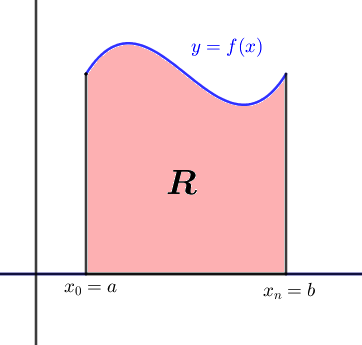
\includegraphics[width=.3\textwidth]{imagenes/imagenes08/T08IM01.png}
	\end{figure}
	
\end{multicols}

\begin{multicols}{2}

Hacemos una `Partición' del intervalo  $[a,b]: \quad \left\{ P=  x_0=a, x_1, x_2, \cdots , x_n=b \right\}$

$A(R)=\sum _{ i=1 }^{ n }{ A(R\_ i) } \; $  (A=área)

El área del trapecio mixtilíneo $R_i$ está comprendida entre dos rectángulos de base $(x_{i+1}-x_{i})$ y de alturas de alturas $M_i$ y $m_i$, valores máximo y mínimo de $f(x)$ en $[x_{i-1}, x_i]$ (que no tienen que coincidir con los límites del intervalo $[x_{i}, x_{i+1}]$ como aparece en la figura adjunta), Así:



 	\begin{figure}[H]
		\centering
		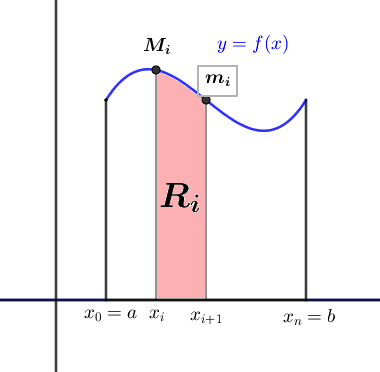
\includegraphics[width=.4\textwidth]{imagenes/imagenes08/T08IM02.png}
	\end{figure}
\end{multicols}
$ m_i\cdot (x_i-x_{i-1}) \le A(R_i) \le M_i\cdot (x_i-x_{i-1})$

Sumando, $=\sum _{ i=1 }^{ n }$, tendremos $L(f,P)\le A(R) \le U(f,p)$, Siendo $L$ una aproximación al área por defecto (lower) y $U$ una aproximación por exceso (upper).

$L(f,P)=\sum _{ i=1 }^{ n }{ m_i\cdot \left( { x }_{ i }-{ x }_{ i-1 } \right)  } \; \le A(R) \le  \;  U(f,P)=\sum _{ i=1 }^{ n }{ M_i\cdot \left( { x }_{ i }-{ x }_{ i-1 } \right)  } $

Al hacer la partición más `fina' (dividir $[a,b]$ en más rectángulos más pequeños, la aproximación mejora. 

También se puede mejorar la aproximación si en cada $A(R_i)$, en vez de tomar $M_i$ o $m_i$, tomamos un valor intermedio. 
\begin{figure}[H]
	\centering
	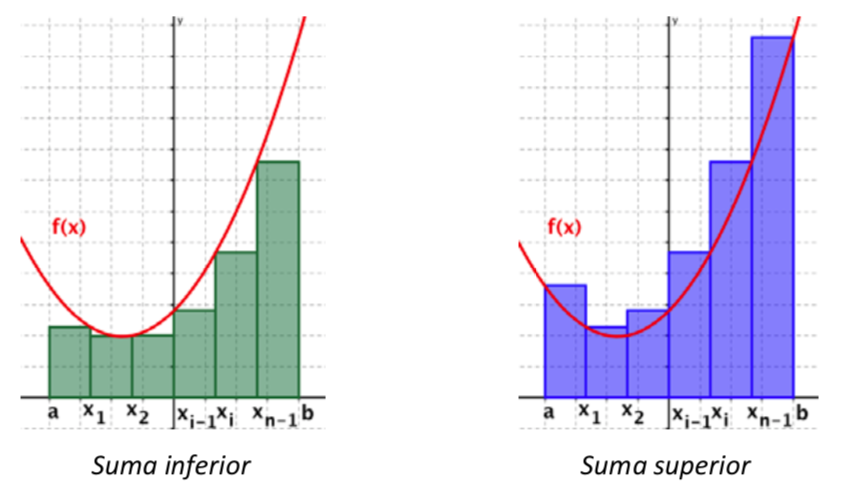
\includegraphics[width=.7\textwidth]{imagenes/imagenes08/T08IM09.png}
\end{figure}


\subsection{Integral de una función continua}

\begin{defi} Integral Definida.

Sea $y=f(x)$ una función continua y positiva en $[a,b]$ . Sea R el trapecio mixtilíneo determinado por $f(x)$, las rectas $x=a$,  $x=b$ y el eje $OX$. Al área de este trapecio mixtilíneo $A(R)$ le llamamos integral definida de $f(x)$ desde $x=a$ hasta  $x=b$  con el eje $OX$, que denotamos por:$\; \; \boxed{\displaystyle \; A(R) = \; \int_a^b f(x)\; \dd x \;= \int_a^b f(t)\; \dd t\; \  }\quad $ $a$ y $b$ son los llamados \emph{`límites de integración'}.
	
\end{defi}

\begin{multicols}{2}

\underline {$\divideontimes$ Procedimiento para el cálculo de}  $\displaystyle \; \int_a^b f(x)\; \dd x \; $

\begin{figure}[H]
	\centering
	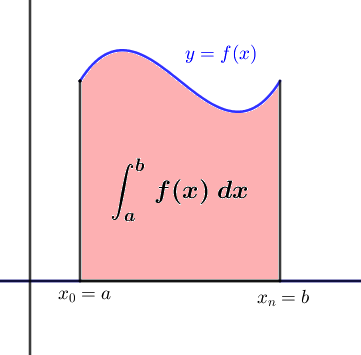
\includegraphics[width=.4\textwidth]{imagenes/imagenes08/T08IM03.png}
\end{figure}

\begin{enumerate}[1.- ]
	\item Tomamos una partición del intervalo: $P\; \equiv \; a=x_0<x_1<x_2< \cdots <b=x_n$
	\item A la mayor de las distancias $x_{i+i}-x_i$ le llamamos `norma' o diámetro de $P$.
	\item A cada partición le asociamos un área por defecto, $L(f,P)$ y una por exceso, $U(f,P)$. estas áreas cumplen, evidentemente, que:
	$L(f,P) < A(R)= \displaystyle \; \int_a^b f(x)\; \dd x < U(f,P)$
	\item Supongamos que tenemos una sucesiones de particiones $P_1, P_2, P_3, \cdots , P_k, \cdots \; $ a las que les corresponderán una sucesión de áreas por defecto $L_1, L_2, \cdots \; $ y otra por exceso $U_1, U_2, \cdots \; $.
	\item Si los diámetros de las particiones tienden a cero (cada partición es `más fina' que la anterior) entonces, se puede demostrar que la sucesión de diferencia de áreas de cada partición, $U_1-L_1, U_2-L_2, \cdots , U_k-L_k, \cdots \; $, también tiende a cero. Luego ambas sucesiones tienden al área buscada (criterio del sandwich de límites, teorema \ref{teor:Sandwich})
	
	$\displaystyle  L_k\le \int_a^b f(x)\; \dd x \le U_k \; $ Si para todo $k$ se cumple que $\underset {k\to 0}{lim}\; {U_k-L_k}=0 \Rightarrow \quad$
	
	\centerline{$\boxed{\; \displaystyle Uk \rightarrow \int_a^b f(x)\; \dd x \leftarrow L_k \;} $}
	
	\item Si ambas sucesiones tienden a este límite $\left( \; \displaystyle \int_a^b f(x)\; \dd x \; \right)$, también lo hará cualquier otra sucesión cuyos términos se formen del siguiente modo:
	$\displaystyle \sum _{ i=1 }^{ n }{ ({ x }_{ i }-{ x }_{ i-1 })\cdot f({ c }_{ i }) } \; $, ya que $m_i\le f(c_i)\le M_i$, con $c_i\in [x{i-1},x_i]$. Es decir: $L_k\le S_k\le U_k$
	
\end{enumerate}
\end{multicols}

\vspace{4mm}

\underline{$\divideontimes$ Resumen práctico:}


Para calcula la integral definida de una función continua $f(x)$ entre $x=a$ y $x=b$ con el eje $OX$, haremos lo siguiente:

\begin{enumerate}[a) ]
	\item Construir una sucesión de particiones cada ves más fina (que la norma o diámetro tienda a cero).
	\vspace{-3mm} \item Elegir en cada intervalo un punto $c_i$
	\vspace{-3mm} \item Obtener el término de la sucesión: $\displaystyle S_n= \sum _{ i=1 }^{ n }{ ({ x }_{ i }-{ x }_{ i-1 })\cdot f({ c }_{ i }) } \; $
	\vspace{-3mm} \item Calcular $\displaystyle \underset {n\to \infty}{lim}\; {S_n}=  \int_a^b f(x)\; \dd x$
\end{enumerate}


\begin{ejem}
\label{trapecio-mixtilineo}
	$\divideontimes$ Calcular. $\displaystyle \int_0^2 (2x+1) \; \dd x$
\begin{multicols}{2}	
	\begin{figure}[H]
	\centering
	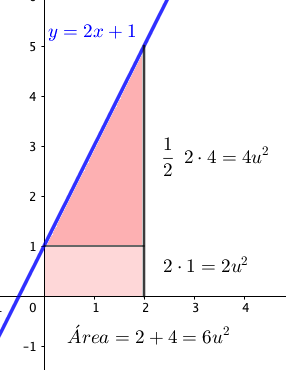
\includegraphics[width=.3\textwidth]{imagenes/imagenes08/T08IM04.png}
\end{figure}
	$[0,2] \to 2/n \Rightarrow P_n\; \equiv \; x_0=0, x_1=2/n; x_2=4/n; x_3= 8/n; \cdots ; x_k=2k/n; \cdots ; x_n=2n/n=2 $
	
	$\displaystyle { S }_{ n }=\sum _{ i=1 }^{ n }{ \frac { 2 }{ n }  } \cdot \left( 2\left( \frac { 2i }{ n } +1 \right)  \right) = \frac { 2 }{ n } \left[ \frac { 4 }{ n } \sum _{ i=1 }^{ n }{ i } +\sum _{ i=1 }^{ n }{ 1 }  \right] =\left( P.A. \right) $
	
	$= \displaystyle \frac { 2 }{ n } \left[ \frac { 4 }{ n } \frac { (1+n)\cdot 2 }{ 2 } +n \right]$
	
	$ =\displaystyle \frac { 2 }{ n } \left[ 2\left( 1+n \right) +n \right] =\frac { 6n+4 }{ n } $
\end{multicols}
$\displaystyle \int_a^b f(x)\; \dd x = \underset {n\to \infty}{lim}{Sn}=\displaystyle \underset {n\to \infty}{lim}{\dfrac {6n+4}{9}}= 6$
\end{ejem}

\vspace{4mm}

\underline{Observación}: Si calculamos  $\displaystyle \int_0^2 (-x+2) \dd x =\textcolor{gris}{[1-1]}=0  \neq \text { area } $ , pues $f(x)$ no es positiva en $[0,2]$

 \begin{multicols}{2}

 Si $f(x)\ge 0 $ en $[a,b]$, entonces $\displaystyle \int_a^b f(x)\; \dd x $ representa el área de $f(x)$, en $[a,b]$, con eje $OX$ (\textcolor{gris}{área=$|1|+|-1|=2u^2$}), pero si $f(x) \ngeq  0 $, entonces $\displaystyle \int_a^b f(x)\; \dd x $  no representa ningún área. Aprenderemos a calcular áreas de funciones con el eje $OX$ en secciones posteriores.
 
 Lo único claro, de momento, es que $\displaystyle \int_a^b f(x)\; \dd x \; \in \; \mathbb R $ 
	
	\begin{figure}[H]
	\centering
	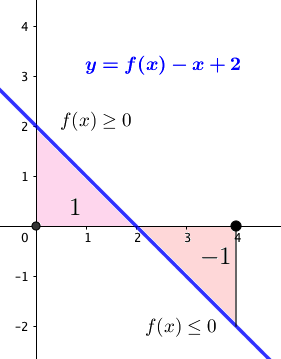
\includegraphics[width=.35\textwidth]{imagenes/imagenes08/T08IM05.png}
	\end{figure}
	\end{multicols}



-- Pero, ?`qué es la integral definida?

-- Pues una \emph {`suma' } de (muchos) infinitos términos (muy pequeños) infinitesimales. 
	
\subsection{Propiedades de la integral definida} 
$f(x)$ ctna. en $[a,b]$

\begin{enumerate}
	\item $\boxed{\; \displaystyle \int_a^a f(x)\; \dd x = 0 \; }$. 

	Rectángulos mixtilíneos de base $0$
	
	\item Si $a>b \to \quad $   $\boxed{ \; \displaystyle \int_a^b f(x)\; \dd x =-\displaystyle \int_b^a f(x)\; \dd x \; }$ 
	
	Efectivamente, las bases de los rectángulos son ahora negativas: $(x_i-x_{i-1})=-(x_{i-1}-x_i)$
	
	\item Si $a<c<b \; \; \to \quad$ $\boxed{ \; \displaystyle \int_a^b f(x)\; \dd x = \int_a^c f(x)\; \dd x +\int_c^b f(x)\; \dd x \; }$ 
	
	Esta propiedad es evidente pensando que $f$ es positiva en todo  $[a,b]$, si $c\in ]a,b[$, entonces el área desde $a$ hasta $b$ coincide con la suma de las áreas desde $a$ hasta $c$ y desde $c$ hasta $b$.
	
	\item $f$ ctna. en $]a,b[\; \;$ y existen:$\quad \underset{x\to a^+}{lim}\;{f(x)}=\alpha \quad \text {y} \quad \underset{x\to b^-}{lim}\;{f(x)}=\beta $,
	
	definimos: $f_1(x)=\begin{cases}
				\alpha & x=a \\
				f(x) & a<x<b \\
				\beta & x=b
				\end{cases} \quad \Rightarrow \displaystyle \quad \int_a^b f(x)\; \dd x=\displaystyle \int_a^b f_1(x)\; \dd x$
	
	\begin{multicols}{2}
	
	Como muestra la imagen, para el área desde $a$ hasta $b$ no importa que la función no sea continua en los extremos del intervalo, llamados `límites de integración'. 
	
	\begin{figure}[H]
	\centering
	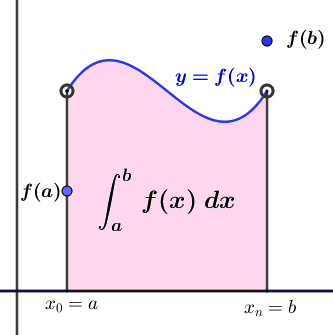
\includegraphics[width=.25\textwidth]{imagenes/imagenes08/T08IM06.png}
	\end{figure}
	\end{multicols}
	
	\vspace{-3mm} \emph{Las propiedades $3$ y $4$ permiten extender el concepto de integral definida (ID) a funciones definidas a trozos, incluso con discontinuidades finitas (discont. de salto y evitables). }
	
	\item \underline{Linealidad de la ID} : Sea $\alpha, \beta \in \mathbb R$\; , $f\; $ y $g\; $ ctnas. en $[a,b]\; $, entonces:
	
	\hspace{15mm} $\boxed{ \; \displaystyle \int_a^b \left(\alpha \cdot f(x) \pm \beta \cdot g(x)  \right)\; \dd x = \alpha \; \int_a^b f(x)\; \dd x +\beta \;  \int_a^b g(x)\; \dd x \; } $
	
	\textcolor{gris}{ (Esta propiedad la damos sin justificación, será evidente después del th. fundamental del cálculo y de la regla de Barrow.)}
\end{enumerate}

\subsection{El teorema de la media}

\begin{teor}{Teorema de la media o th. del valor medio del cálculo integral.}

$f\; $ ctna. en $[a,b]\; \to \; \exists \; c \; \in \; ]a,b[ \;\;  \therefore  \; \displaystyle \int_a^b f(x)\; \dd x = f(c)\cdot (b-a)\; $
\end{teor}

\underline{Aplicación:} Valor medio de una función continua en un intervalo:

Si $f\;$ es integrable en $[a,b]\; $, se llama VALOR MEDIO de $f\; $ en  $[a,b]\; $ al valor:

$\; <\; f \; > = \dfrac {1}{b-a }\cdot \displaystyle \int_a^b f(x)\; \dd x \; $
\begin{multicols}{2}
\underline{Interpretación geométrica:} 

$ \exists \; c \; \in \; ]a,b[ \;$ tal que él área encerrada bajo la curva $y=f(x)\; $ (supuesta $f(x)\ge 0$) con $OX\; $ en $[a,b]\; $ coincide con el área de un rectángulo de base $b-a\;$ y altura comprendida entre en Máximo y el mínimo de $f\; $ en $[a,b]\; $. Como muestra la figura adjunta.

\begin{figure}[H]
 	\centering
	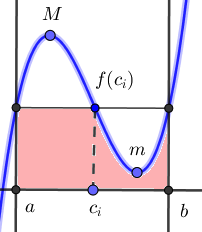
\includegraphics[width=.25\textwidth]{imagenes/imagenes08/T08IM07.png}
\end{figure}
\end{multicols}



\begin{proof} 
Nos basamos en los teoremas vistos en la sección de `propiedades de las funciones continuas en intervalos cerrados', sección \ref{prop-func-ctnas}.

Como $f$ en ctna. en $[a,b]$, alcanza en algunos de los puntos del intervalo un valor máximo $M$ y uno mínimo $m$, por lo que:
$\quad m(b-a) \le \displaystyle \int_a^b f(x) \dd x \le M(b-a)$

Es decir, $\quad m \; \le\;  \dfrac {1}{b-a}\displaystyle \int_a^b f(x) \dd x \; \le\;  M \; \;$. Puesto que $f$ es ctna., debe existir un $c\in]a,b[$ para el cual la función alcanza este valor comprendido entre el $M$ y el $m$:

$\exists \; c \; \in \; ]a,b[ \quad  \therefore  \quad  f(c)= \dfrac {1}{b-a }\cdot \displaystyle \int_a^b f(x)\; \dd x \quad $ .  A este valor se le llama `valor promedio de $f$ en $[a,b]$'.
\end{proof}

\begin{ejem}
En el ejemplo \ref{trapecio-mixtilineo}, vimos $\displaystyle \int_0^2 (2x+1) \; \dd x=6=f(c)\cdot 2$, con $c\in [0,2]$. Luego $f(c)=6/2=3 =2c+1 \to c=1 \in [0,2]$

$<f>=\dfrac{1}{2-0} \displaystyle \int_0^2 (2x+1) \; \dd x = \frac 1 2 \cdot 6 = 3 $, que es el valor promedio de $y=2x+1$ en $[0,2]$.
\end{ejem}

\begin{ejem}$\divideontimes$
Demostrar que $\underset{t\to 0^+}{lim}\;{\dfrac 1 t \; \displaystyle \int_{t^2}^t \dfrac {\sin x}{x}\; \dd x }=1$

Como $0\notin [t^2,t],\quad f(x):\dfrac {\sin x}{x}\;$ es ctna. Aplicamos el TVM CI (teorema del valor medio del cálculo integral):

$\displaystyle \displaystyle \int_{t^2}^t \dfrac {\sin x}{x}\; \dd x =f(c)\cdot (t-t^2)= \dfrac {\sin c}{c} 	\cdot (t-t^2)$, con $c\in[t^2,t]$

Si $t\to 0^+ \rightarrow c\to 0^+$, además $\underset{c\to 0^+}{lim}\;{\dfrac {\sin x}{x}}= [\text { L'H }]= 1$, entonces:

$\underset{t\to 0^+}{lim}\;{\dfrac 1 t \; \displaystyle \int_{t^2}^t \dfrac {\sin x}{x}\; \dd x }= \underset {t \to 0^+}{lim}\; {\dfrac 1 t \cancelto{1}{\dfrac {\sin c}{c}} (t^2-t) } =\underset {t\to 0^+}{lim}\; {\dfrac {\cancel{t}(1-t)}{\cancel{t}}}=1$
\end{ejem}


\section{Relación entre integral y derivada}
\subsection{El Teorema fundamental del cálculo integral. Corolarios}

\begin{multicols}{2}
\begin{defi} `Función Área'

$f$ ctna. en $[a,b]$ , $\forall x \in [a,b]$, definimos:

$F(x)=\displaystyle \int_a^x f(t)\; \dd t$

Para cada $x \in [a,b]$, $F(x)$ mide el área desde $a$ hasta $x$ de $f(x)$ con $OX$ (supuesta $f(x)\ge 0$)
\begin{figure}[H]
 	\centering
	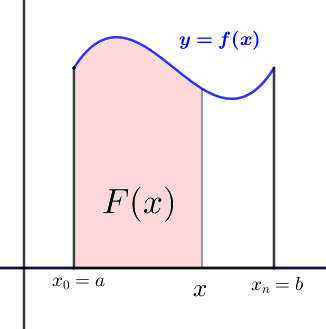
\includegraphics[width=.35\textwidth]{imagenes/imagenes08/T08IM08.png}
\end{figure}	
\end{defi}
\end{multicols}

\begin{teor} {``Teorema Fundamental del Cálculo Integral''}
\label{TFCI}
	$f$ ctna. en $[a,b]$ y sea $\displaystyle F(x)=\int_a^x f(t) \dd t$, entonces:

\hspace{25mm} $F(x)$ es derivable y, además, $F'(x)=f(x)$
\end{teor}

\begin{proof}
	Calculemos $F'(x)=\underset{h\to 0}{lim}\; {\dfrac {F(x+h)-F(x)}{h}}= \displaystyle \underset{h\to 0}{lim}\; {\dfrac {\int_a^{x+h}f(t) \dd t - \int_a^x f(t) \dd t}{h}} =$
	
	Aplicando la Propiedad 3 de la ID vista anteriormente:
	
	$= \displaystyle \underset{h\to 0}{lim}\; {\dfrac { \left( \cancel{\int_a^{x}f(t) \dd t} + \int_x^{x+h} f(t) \dd t\right) - \cancel{\int_a^x f(t) \dd t}}{h}} = \displaystyle \underset{h\to 0}{lim}\;\;  {\dfrac { \int_x^{x+h} f(t) \dd t}{h}} = \; \to $
	
	Como $f$ ctna. en $[a,b]$ y $x, x+h \; \in [a,b]$, entonces, $f$ ctna en $[x,x+h]$. Aplicando el TVM del Cálculo Integral:
	
	$\exists c\in [x,x+h] \;\;  \therefore  \; \displaystyle \int_x^{x+h} f(t) \dd t\; = \;  \left( (\cancel{x}+h)-(\cancel{x}) \right)\cdot f(c)=h\cdot f(c)$, luego:
	
	$\displaystyle \to \; = \underset{h\to 0}{lim}\;\;  {\dfrac {\cancel{h} \cdot f(c)}{\cancel{h}}} = \underset{h\to 0}{lim}\;{f(c)} = \left\{
	 \; c \in [x,x+h]  \quad h\to 0 \Rightarrow c\to x  
	 \right\}= f(x)$	
\end{proof}

	 Luego $\textbf{F'(x)=f(x)}$. Es decir La función área $F(x)$ es derivable y su derivada vale el integrando $f(x)$. \underline{Asombrosamente}, esta relación \emph{liga} el cálculo integral (cálculo de áreas) con la derivación (búsqueda de rectas tangentes), lo cual abre un gran abanico de posibilidades teórico-prácticas en matemáticas.
	 
	 Este es el motivo por el cual al cálculo de anti-derivadas o primitivas le llamamos cálculo integral indefinida) y por eso usábamos la extraña notación $\int f(x) \dd x$.
	 
	 El símbolo $\displaystyle \int$ para representar a la integral fue introducido por Euler, a finales del XVII e intenta asimiliarse a una ese  alargada, pues la integral definida no es más que una \underline{s}uma de infinitos infinitésimos.

\subsection{La regla de Barrow}
% $\eval[x|_0^\infty$.   $\eval{x}_0^\infty$ $\left[ x \right|_a^b $

\begin{teor}{La regla de Barrow}
\label{Barrrow}

Sea $f(x)$ una función ctna. en $[a,b]$ y sea $F(x)$ una primitiva de $f(x)$ ($F'(x)=f(x)$) 

$\longrightarrow \quad \displaystyle \boxed{ \; \int_a^b f(x)\; \dd x = \eval[f(x)|_a^b = F(b)-F(a)\;}  \quad \in \; \mathbb R$ 	
\end{teor}

\begin{proof}
	Por el Tf. Fundamental del Cálculo Integral, teorema \ref{TFCI}, $\displaystyle G(x)=\int_a^x f(t)\; \dd t$, con $G'(x)=f(x)\; $. 
	
	Si $F(x)$ es otra primitiva cualquiera de $f(x)$, por el corolario \ref{teor:fdmtalCI} visto en el tema de 	\ref{AplicDeriv} `Aplicaciones de las derivadas': $F(x)=G(x)+\mathcal C$ (dos funciones, con la misma derivada, difieren en una constante).
	
	$\circ \;$ En $\displaystyle x=a \longrightarrow G(a)=\int_a^a f(t)\; \dd t=0 = (\text {Prop. 1 ID}) = F(a)+\mathcal C \longrightarrow \mathcal C=-F(a)$
	
	$\circ \;$ En $\displaystyle x=b \longrightarrow G(b)=\int_a^b f(t) \; \dd t=F(b)+\mathcal C =$
	( \tiny{sustituyendo el valor de} $ \mathcal C\;  $ ) \normalsize {$=F(b)-F(a)$} 
	
	Por lo que $\displaystyle \int_a^b f(t)\; \dd t = F(b)-F(a)\; $, con $F$ una primitiva cualquiera de $f$ 
\end{proof}

La importancia de la regla de Barrow es doble:

--- Permite calcular integrales definidas sin necesidad de hallar las sumas de Riemann.

--- Representa una \textbf{conexión} entre el Cálculo Diferencial y el Cálculo Integral. 

\subsection{Corolarios del Teorema fundamental del Cálculo Integral}

Veamos dos aplicaciones del TFCI que, por facilitar la exposición,  daremos sin demostración.

\begin{coro} {Generalización - $1$}

$f(x)$ ctna. en $[a,b]$ y $\displaystyle F(x)=\int_a^{h(x)} f(t)\;  \dd t$, entonces, si $h(x)$ es derivable, se cumple que $F(x)$ es derivale y, además: $\quad  \qquad F'(x)=f(h(x))\cdot h'(x)$
\end{coro}

\begin{coro} {Generalización - $2$}

$f(x$) ctna. en $[a,b]$ y $\displaystyle F(x)=\int_{g(x)}^{h(x)} f(t) \dd t$, entonces, si $g(x)$ y  $h(x)$ son derivables, se cumple que $F(x)$ es derivale y, además: 
$\qquad  \qquad F'(x)=f(h(x))\cdot h'(x)- f(g(x))\cdot g'(x)$	
\end{coro}

\begin{ejem} Calcula: 

$\displaystyle \int_0^2 (2x+1)\; \dd x= \eval[ x^2+x|_0^2 = (2^2+2)-(0)=6$.

 Y ya está, no sabemos más, ni lo que representa ese $6$. Si, por alguna razón, sabemos que $f(x)>0$ en $[0,2]$, la integral sí da $6 u^2$, si no es así, no sabemos interpretar que representa ese resultado.
\end{ejem}

\begin{ejem}
Calcúlese la derivada de la función $F(t)=\displaystyle \int_0^t |x-1|\; \dd x$	

Como $F(t)$ es la función área de $f(x)=|x-1|$, en cualquier $[0,b]; b>0$ esta función es ctna. (y positiva), por lo que su área $F(t)$ será derivable, además, $F'(t)=f(t)=|t-1|$.

(Aunque f(x) no sea dvble. en $x=1$, eso no importa, solo necesitamos que sea ctna).
\end{ejem}




\subsection{Cambio de variable en la integral definida}

Supongamos que mediante la regla de Barrow se desea calcula $I=\displaystyle \int_a^b f(x)\; \dd x$ y que para hallar una primitiva de $f(x)$ necesitamos un cambio de variable $x$ y deshacer luego el CV para aplicar la regla de Barrow. Podemos ahorrar operaciones extendiendo el cambio de variable elegido, $x=g(t)$, a los límites de integración: si
$x=a \to t=g^{-1} (a)$ y si 
$x=b \to t=g^{-1} (b)$. Entonces:

\hspace{15mm} $I=\displaystyle \int_a^b f(x)\; \dd x = [CV x=g(t)] = \int_{g^{-1} (a)}^{g^{-1} (b)} f(g(t))\;  g'(t) \; \dd t$
 
 Siempre que se cumpla:
 
 \hspace{20mm} $1) \quad f \text{ ctna. en  }  g([a,b])$
 
 \hspace{20mm} $2) \quad $ !`Atención: es necesario que  $g(x)$ sea \underline{inyectiva}, 
 
  \hspace{20mm} con derivada ctna. en $\left[ g^{-1} (a),g^{-1} (b) \right] \; $!.

\begin{ejem}
	Calcular $I=\displaystyle \int_0^1 \sqrt{4-x^2}\; \dd x$
	
	$\circ \quad$ PRIMER MÉTODO: Hacemos el CV, integramos, deshacemos el CV y aplicamos Barrow
	
	$\displaystyle \int \sqrt{4-x^2}\; \dd x= [CV: x=2 \sin t]= 2\int \sqrt{1-\sin^2 t} \cdot 2 \cos t\; \dd t= 4\int \cos^2 t \; \dd t = [ \text { fórmula de reducción }]= 4 \int \frac 1 2 \left (1+\cos 2t  \right)\; \dd t  =2t+\sin 2t= [\text { Desh. CV }]= 2 \arcsin (x/2) + \frac 1 2 x \sqrt{4-x^2}+\mathcal C$. Por lo que:
	
	$I=\displaystyle \int_0^1 \sqrt{4-x^2}\; \dd x =\eval [ 2 \arcsin (x/2) + \frac 1 2 x \sqrt{4-x^2} |_0^1= (2 \pi/6 + \frac 1 2 \sqrt{3})-(0-0)=\pi/3 +\frac {\sqrt{3}}{2}$
	
	\vspace{5mm}
	
	$\circ \quad$ SEGUNDO MÉTODO: Extendemos el CV a los límites de integración.
	$I=  \text{ CV: }  
	 \left[ \begin{matrix}
	 x=2\sin t & \dd x=2 \cos t \dd t \\ 
	 x=1 & t=\pi/6 \\ 
	 x=0 & t=0 
	 \end{matrix} \right] = \displaystyle \int_0^{\pi/6} \cos^2 t \; \dd t= \cdots = \eval[2t+\sin 2t|_0^{\pi/6}=\cdots=\pi/3 +\frac {\sqrt{3}}{2}$  
	 
	 Nótese que el cambio elegido, $x=2 \sin t$ sí es INYECTIVA en $[0, \pi/6]$
\end{ejem} 

\begin{ejem}
	Calcula $I=\displaystyle \int_{-1}^1 \dd x$
	
	$I\displaystyle = \eval[x|_{-1}^{1}= 1-(-1)=2$
	
	Pero si hacemos el CV $x^2=t \to 2 x\;  \dd x= \dd t\to   	\dd x = \dfrac {1}{\sqrt t}\; \dd t $
	
	$x=-1 \to t=(-1)^2=1; \quad x=1 \to t=(1)^2=1$, entonces:
	
	$I=\displaystyle \int_1^1 \dfrac {1}{\sqrt t}\; \dd t = 0$, por la propiedad $1$ de las integrales definidas. ?`Dónde está el fallo?'
	
	\rotatebox{180}{\leftline{\textcolor{gris}{¡Ojo:  $x=t^2$ \underline{no es inyectiva} en $[-1.1]\; $ !}}}
	
\end{ejem}

\subsection{Integrales impropias}

El concepto de ID puede extenderse a límites de integración infinitos del siguiente modo:
$\quad \displaystyle \int_a^{+\infty} f(t)\; \dd t = \underset{x\to + \infty}{lim}\;{\int_a^x f(t)\; \dd t}$

\begin{ejem}
Calcula: $a) \quad \displaystyle \int_1^{+\infty} \dfrac {1}{t^2} \dd t\; ; \qquad \quad b) \quad \displaystyle \int_1^{+\infty} \dfrac 1 t \dd t $	

$a)\quad \displaystyle \int_1^x \dfrac {1}{t^2} \dd t= \eval[-\dfrac{1}{x}|_1^x=-\dfrac 1 x + 1 \Rightarrow \; \;  \displaystyle \int_0^{+\infty} \dfrac {1}{t^2}\; \dd t = \underset{x\to + \infty}{lim}\;{-\dfrac 1 x + 1}=1$

$b) \quad \displaystyle \int_1^x \dfrac 1 t \dd t = \eval[\mathrm{ln}\abs{x}|_1^x=\mathrm{ln}x-\cancelto{0}{\mathrm{ln}1}=\mathrm{ln}x \Rightarrow \;\; \displaystyle \int_1^{+\infty} \dfrac {1}{t}\; \dd t = \underset{x\to + \infty}{lim}\;{\mathrm{ln}x}=+\infty$

\begin{figure}[H]
 	\centering
	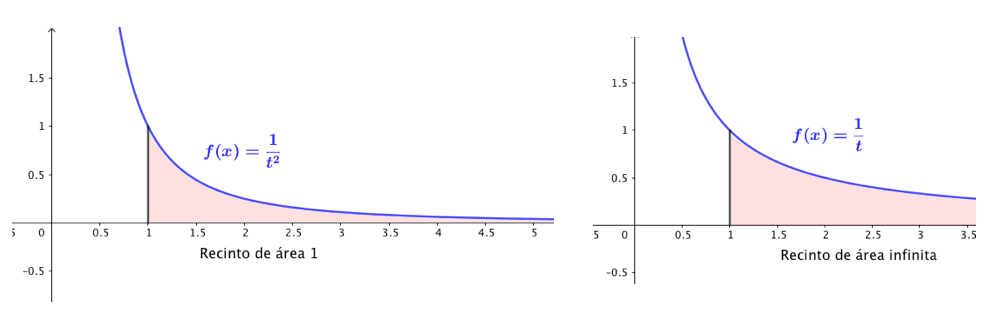
\includegraphics[width=1\textwidth]{imagenes/imagenes08/T08IM10.png}
\end{figure}

\end{ejem}

\vspace{-4mm} \textbf{Otras integrales impropias:}

Si $f$ no está acotada en $[a,b]$ (discontinuidad asintótica o de salto infinito), en general, la $\displaystyle \int_a^b f(t) \dd t$ no existe. Sin embargo, en algunos casos, se puede proceder de forma análoga al caso anterior. Si por ejemplo $f$ presenta una discontinuidad de salto infinito en $c\in[a,b]$:

$\displaystyle \int_a^b f(t) \dd t= \underset {x\to c^-}{lim}{\int_a^x f(t) \dd t}-\underset {x\to c^+}{lim}{\int_x^b f(t) \dd t}$


\begin{ejem}
Calcula: $a) \quad \displaystyle \int_0^1 \dfrac {1}{\sqrt{t}} \dd t\; ; \qquad \quad b) \quad \displaystyle \int_0^1 \dfrac {1} {t^2} \dd t $	

$a) \quad \displaystyle \int_0^1 \dfrac {1}{\sqrt{t}} \dd t= \underset {x\to 0^+}{lim}{\int_x^1 \dfrac {1}{\sqrt{t}} \dd t} =\underset {x\to 0^+}{lim} { \eval[2\sqrt{t}|_x^1 }= \underset {x\to 0^+}{lim} {2-2\sqrt{x}}=2$

$b) \quad  \displaystyle \int_0^1 \dfrac {1} {t^2} \dd t = \underset {x\to 0^+}{lim}{\int_x^1 \dfrac {1}{t^2} \dd t}= \underset {x\to 0^+}{lim} { \eval[-\dfrac 1 t|_x^1 }=\underset {x\to 0^+}{lim} {\left(-1+\dfrac 1 x  \right)}=+\infty$

\begin{figure}[H]
 	\centering
	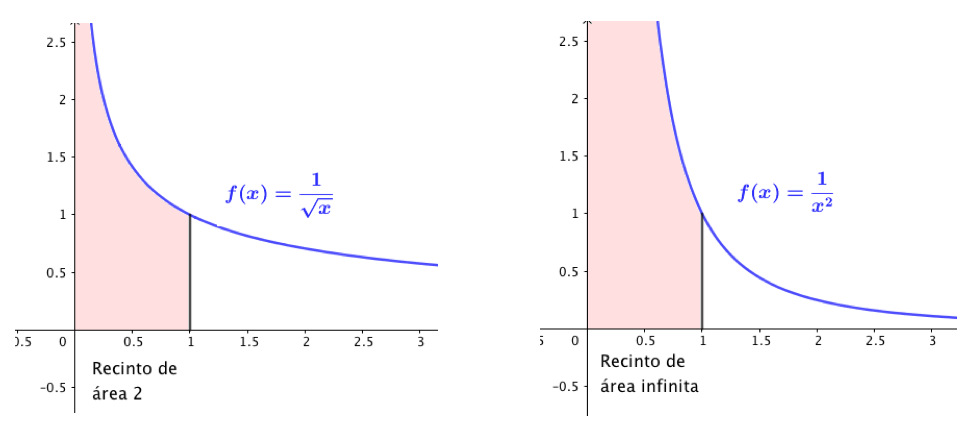
\includegraphics[width=0.9\textwidth]{imagenes/imagenes08/T08IM11.png}
\end{figure}

\end{ejem}

Resumiendo:

En cálculo, una integral impropia es el límite de una integral definida cuando uno o ambos extremos del intervalo de integración se acercan a un número NO real específico,  o a $\pm \infty$.

Además una integral definida es impropia cuando la función integrando de la integral definida tiene discontinuidad infinita en el intervalo de integración. 

También se pueden dar ambas situaciones.


\subsection{Ejercicios de Integrales definidas}

% $\eval[x|_a^b$.   $\eval{x}_0^\infty$ $\left[ x \right|_a^b $
--- \textbf{Ejercicios resueltos de Integral Definida.}

\begin{ejre}
$\divideontimes \; \; $Utilizando sumas de Riemann, calcúlese la integral de $f(x)=\dfrac 1 3 x$ en el intervalo $[3,5]$.	
\end{ejre}

\begin{proofw}\renewcommand{\qedsymbol}{$\diamond$}	

 Sea $P_n$ la partición obtenida al dividir el intervalo $[3,5]$	 en $n$ partes iguales. Como la amplitud del intervalo es $5-3=2$, cada subintervalo tendrá amplitud $2/n$, con lo que se cumplirá que $\underset{n\to +\infty}{lim}{\dfrac 2 n}= 0$	

$P_n=\left\{ x_0=3, x_1=3+2/n, x_2=3+4/n, \cdots, x_n=3+2n/n=5   \right\}$

En cada intervalo $[x_{i-1}, x_i]$ tomaremos $c_i=3+i\cdot \dfrac 2 n$, con lo que la suma de Riemann será:

$S(f,P)=\displaystyle \sum _{ i=1 }^{ n }{ f(c_i) \cdot (x_i-x_{i-1}) } = \sum _{ i=1 }^{ n } {\frac 1 3 \left( 3+i\cdot \frac 2 n  \right) \; \frac 2 n} = \frac {2}{3n} \sum _{ i=1 }^{ n } {\left( 3+i\cdot \frac 2 n  \right)} =$

$= \displaystyle \frac {2}{3n} \left( \sum _{ i=1 }^{ n }{3} + \frac 2 n \sum _{ i=1 }^{ n }{i}  \right) = \frac {2}{3n} \left( 3n + \frac 2 n \cdot \frac {(1+n)\; n}{2} \right)= 2 + \dfrac {2n+2}{3n}$

Entonces, $\displaystyle \int_3^5 f(x)\; \dd x= \underset {n\to +\infty}{lim}{2+ \dfrac {2n+2}{3n}}=1+\frac 2 3 = \frac 8 3$

\end{proofw}

\begin{ejre}
Sea $\displaystyle F(x)=\int_0^x \mathrm{ln} (t^2+4t)\; \dd t$. Calcula $F'(x)$	
\end{ejre}
\begin{proofw}\renewcommand{\qedsymbol}{$\diamond$}	
	
	Por el primer corolario del th. fundamental del cálculo integral, siendo $\mathrm{ln} (t^2+4)$ continua:
	$\quad F'(x)=\mathrm{ln} (t^2+4)$
\end{proofw}



\begin{ejre}
 Aplicar el TVM del cálculo integral a la función $f(x)=x^2+x+1$ en el intervalo $[1,4]$ y calcúlese el valor medio de $f$ en dicho intervalo.
\end{ejre}

\begin{proofw}\renewcommand{\qedsymbol}{$\diamond$}	

Como $f\; $ ctna. en $[1,4]\; \to \; \exists \; c \; \in \; ]1,4[ \;\;  \therefore  \; \displaystyle \int_1^4 f(x)\; \dd x = f(c)\cdot (4-1)\; $

$\displaystyle \int_1^4 (x^2+x+1)\; \dd x =\eval[\frac {x^3}{3}+\frac {x^2}{2}+x|_1^4 = \cdots = \frac {63}{2}$ 

Busquemos el $c$ del th.: $\exists c \in [1,4] \; / \; f(c)=\frac {21}{2} \to c^2+c+1=\frac {21}{2} \to 2c^2+2c-19=0 \to c=\dfrac {-1\pm \sqrt{39}}{2} $, para que esté en el intervalo: $c= \dfrac {-1+ \sqrt{39}}{2} \simeq 2.6\cdots \in ]1,4[ $

\vspace{2mm}El valor medio de $f$ en $[1,4]$ es $<\; f\; >\; =\; \frac 1 3\;  \frac {63}{2}= \frac {21}{2}$ 
	
\end{proofw}

\begin{ejre}$\divideontimes \; \; $ Si $f$ está acotada en $[a,b]$ u es discontinua de salto en un número finito de puntos $\alpha_1<\alpha_2<\alpha_3<\cdots\alpha_m$, entonces, es integrable y si integral vale:

$\displaystyle \int_a^b f(x) \dd x= \int_a^{\alpha_1} f(x) \dd x + \int_{\alpha_1}^{\alpha_2} f(x) \dd x+ \int_{\alpha_2}^{\alpha_3} f(x) \dd x + \cdots + \int_{\alpha_n}^b f(x) \dd x$

Utilícese esto para calcular: $\displaystyle \int_1^3 x^{\left\lfloor x \right\rfloor }\; e^x \; \dd x \; \; $, donde $\left\lfloor x \right\rfloor=E(x)=Int(x)$ es la parte entera de $x$.
	
\end{ejre}

\begin{proofw}\renewcommand{\qedsymbol}{$\diamond$}	

$f(x) = \left\lfloor x \right\rfloor \; e^x =
\begin{cases}	
 x\; e^x & 1\le x<2 \\
 x^2 \; e^x & 2\le x <3 \\
 27 e & x=3	
\end{cases}\quad$. $\quad$ Así pues,:

$\displaystyle \int_1^3 x^{\left\lfloor x \right\rfloor }\; e^x \; \dd x \; \; = \int_1^2 x\; e^x\; \dd x + \int_2^3 x^2\; e^x\; \dd x + \cancelto{0}{\int_3^3 27 e^x\; \dd x}= \cdots =$ (hay que integrar por partes, una vez la primera integral y dos veces en la segunda) $=\cdots= 5e^3-e^2$

\end{proofw}

\begin{ejre}
Calculas las siguientes ID:
\begin{multicols}{2}
\begin{enumerate}[a) ]
\item $\displaystyle \int_0^1 e^x \; \dd x$
\item $\displaystyle \int_{-1}^1 (x+2x^2-x^3+5x^4) \; \dd x$
\item $\displaystyle \int_2^3 \dfrac {1}{\sqrt{x-1}} \; \dd x$
\item $\displaystyle \int_0^{2\pi} \sin x \; \dd x$
\item $\displaystyle \int_2^5 \dfrac {1}{x^2+x-2} \; \dd x$	
\item $\displaystyle \int_0^1 \dfrac {x}{1+x^4} \; \dd x$
\end{enumerate}
\end{multicols}
\end{ejre}

\begin{proofw}\renewcommand{\qedsymbol}{$\diamond$}	


\hspace{5mm} $a) \qquad \displaystyle \int_0^1 e^x \; \dd x = \eval[e^x|_0^1=e^1-e^0=e-1$

$b) \qquad \displaystyle \int_{-1}^1 (x+2x^2-x^3+5x^4) \; \dd x= \eval[ \dfrac {x^2}{2}+\dfrac {2x^3}{3}-\dfrac {x^4}{4}+\dfrac {\cancel{5}x^5}{\cancel{5}}|_{-1}^1  $
$=\left(\dfrac 1 2 + \dfrac  2 3 - \dfrac 1 4 +1 \right) - \left( \dfrac 1 2- \dfrac  2 3 - \dfrac  1 4 - 1   \right)= \dfrac 2 3 + 1 + \dfrac  2 3 + 1 = \dfrac {10} {3}$

$c) \qquad \displaystyle \int_2^3 \dfrac {1}{\sqrt{x-1}} \; \dd x =  \int_2^3 (x-1)^{-1/2} \; \dd x = \eval[2\sqrt{x-1}|_2^3 = 2\sqrt{2}-2$

$d) \qquad \displaystyle \int_0^{2\pi} \sin x \; \dd x= 
\eval[-\cos x|_0^{2\pi}= -1-(-1)=-1+1=0$

$e) \qquad \displaystyle \int_2^5 \dfrac {1}{x^2+x-2} \; \dd x = \displaystyle \int_2^5 \dfrac {1}{(x-1)(x-2)} \; \dd x = \to \; \;$	Tenemos uns integral racional, busquemos una primitiva:

$\displaystyle \dfrac {1}{(x-1)(x-2)}=\frac{A}{x-1}+\frac{B}{x+2}=\frac{A(x+2)+B(x-1)}{(x-1)(x+2)} \Rightarrow $
$\displaystyle \Rightarrow \begin{cases}
 	x=1 \to 1=3A \\
 	x=-2\to -1=-3B	
 \end{cases} \Rightarrow A=-B=1/3 \Rightarrow \int \dfrac {1/3}{x-1}\; \dd x +\int \dfrac {-1/3}{x+2} \; \dd x = \frac 1 3 \mathrm{ln}|x-1| -\frac{1}{3} \mathrm{ln} \abs{x+2} + \mathcal C= \frac 1 3 \left[\mathrm{ln}|x-1|-\mathrm{ln} \abs{x+2}   \right]$. Ya podemos volver a nuestra integral definida:
 
$\to = \displaystyle  \frac 1 3\eval[\;\mathrm{ln} \abs{x-1} - \mathrm{ln} \abs{x+2}\; |_0^1= \cdots = \frac 2 3 \mathrm{ln} 4 - \frac 1 3 \mathrm{ln} 7$

$f) \qquad \displaystyle \int_0^1 \dfrac {x}{1+x^4} \; \dd x = \dfrac 1 2 \int_0^1 \dfrac {2x}{1+(x^2)^2} \; \dd x =
\dfrac 1 2 \eval[\arctan(x^2)|_0^1 =$

$= \dfrac 1 2 \left[ (\arctan 1)-(\arctan 0)  \right]=\dfrac 1 2 \; \dfrac {\pi}{4} =  \dfrac {\pi}{8}$
\end{proofw}

\begin{ejre}
Calcula $\displaystyle \int_0^3 |x^2-x|\; \dd x$, 
\end{ejre}
\begin{proofw}\renewcommand{\qedsymbol}{$\diamond$}	

$f(x)=|x^2-x|=\begin{cases}
x^2-x & \text{ si } x<0 \\
-x^2+x & \text{ si } 0\le x < 1 \\
x^2-x & \text{ si } x\ge 1 	
\end{cases}\quad$ Por lo que:

$\displaystyle \int_0^3 |x^2-x|\; \dd x= \int_0^1 (-x^2+x) \; \dd x+\int_1^3 (x^2-x) \; \dd x=\eval[-\dfrac {x^3}{3}+\dfrac{x^2}{2}|_0^1 + \eval[\dfrac {x^3}{3}-\dfrac{x^2}{2}|_1^3= \cdots = \dfrac {29}{6}$	
\end{proofw}

\begin{ejre}
Calcula $\displaystyle \int_0^3 f(x)\; \dd x$, siendo
$f(x)=\begin{cases}
x &  \text{ si } -1\le x \le 1 \\
x^2+1	& \text{ si } 1 < x \le 3
\end{cases}$
	
\end{ejre}
\begin{proofw}\renewcommand{\qedsymbol}{$\diamond$}	

$\displaystyle \int_0^3 f(x)\; \dd x= \int_0^1 x \; \dd x + \int_1^3  (x^2+1)\; \dd x= \eval[\dfrac {x^2}{2}|_0^1 + \eval[\dfrac {x^3}{3}+ x|_1^3 =$

$= \left( (\dfrac 1 2 )- (0) \right)- \left( (9+3)-(\dfrac 1 3 + 1)   \right) = \dfrac {32}{3}$
	
\end{proofw}

\begin{ejre}
	Calcula $\displaystyle \int_0^{\infty} \dfrac {1}{1+x^2}\; \dd x$
\end{ejre}
\begin{proofw}\renewcommand{\qedsymbol}{$\diamond$}	

$\displaystyle \int \dfrac {1}{1+t^2}\; \dd t = \arctan x + \mathcal C \quad \to \quad \displaystyle \int_0^{\infty} \dfrac {1}{1+x^2}\; \dd x=\eval[\arctan x|_0^{\infty}= $
$\underset {x\to \infty}{lim} \left[ (\arctan x) - (0) \right]$
$=\underset {x\to \infty}{lim}{\arctan x}=\dfrac {\pi}{2}$

\end{proofw}
	
\begin{ejre}
	$\displaystyle \int_0^1 \dfrac 1 x \; \dd x$
\end{ejre}
\begin{proofw}\renewcommand{\qedsymbol}{$\diamond$}	
	
	$\displaystyle \int_x^1 \dfrac 1 x \; \dd x= \eval[\mathrm{ln}\abs {x}|_x^1=  \cancelto{0}{\mathrm{ln} 1}- \mathrm{ln} |x|=-\mathrm{ln} |x| \Rightarrow $
	$\displaystyle \int_0^1 \dfrac 1 x \; \dd x= \underset {x\to 0^+}{lim }{(-\mathrm{ln} x)} =+\infty $
	
	Esta integral ' impropia' es divergente, la integral no existe.
\end{proofw}
% $\eval[x|_a^b$.   $\eval{x}_0^\infty$

\textbf{Ejercicios propuestos de Integral Definida.}

\begin{enumerate} 
\item Resuelve las siguientes ID:

\begin{multicols}{2}
\begin{enumerate}
\item $\displaystyle \int_1^e \dfrac 1 x \; \dd x$
\item $\displaystyle \int_1^2 \dfrac{2x+1}{x^2+x}\; \dd x$
\item $\displaystyle \int_0^{\pi/2} \cos x \: \dd x$
\item $\displaystyle \int_0^7 \dfrac {4}{\sqrt{5x+1}}\; \dd x$
\item $\displaystyle \int_0^1 \arcsin x \; \dd x $
\item $\displaystyle \int_0^{\sqrt{3}} \mathrm{ln} \left(x \sqrt{1+x^2} \right) \; \dd x$
\end{enumerate}	
\end{multicols}


\rightline{\textcolor{gris}{\footnotesize{Solución:$a) \quad 1; \qquad b) \quad \mathrm{ln} 3; \qquad c) \quad 1; \qquad d) \quad 8; \qquad e) \quad \frac {\pi}{2}-1; \qquad f) \quad \mathrm{ln} (\sqrt{2}-1)+\sqrt{2}-1$}}}

\item Resuelve las siguientes ID:

\begin{multicols}{2}
\begin{enumerate}
\item $\displaystyle \int_0^{\infty} \dfrac {1}{x^r}\; \dd x; \text { con } r>1$
\item $\displaystyle \int_2^3 \dfrac {\dd x}{(x-2)^2}  $
\end{enumerate}	
\end{multicols}
\rightline{\textcolor{gris}{Solución: $a) \quad \dfrac {1}{r-1} ; \qquad b) +\infty $}}

\item Calcula	la integral $\displaystyle \int_0^2 f(x)\; \dd x$, siendo $f(x)=\begin{cases}
	x^2 & 0\le x < 1 \\
	2-x & 1\le x \le 2
	\end{cases}$

\rightline{\textcolor{gris}{Solución: $5/6$}}

\item Calcula las derivadas de :
\begin{multicols}{2}
\begin{enumerate}
\item $\displaystyle \int_2^3 \cos^3 t \; \dd t$
\item $\displaystyle \int_x^0 (1+et^2)\; \dd t$
\end{enumerate}	
\end{multicols}
\rightline{\textcolor{gris}{Solución: $a) \quad 0 \; \; (F \text{ es cte. }); \qquad b) \quad -(1+3x^2) \; \; (\; \int_x^0=-\int_0^x \; )$}}

\item Calculas las siguientes ID:
\begin{multicols}{2}
\begin{enumerate}
\item $\displaystyle\int_0^{\dfrac {\mathrm{ln} 2}{3}}  \dfrac {e^x}{1+2e^x}\; \dd x$
\item $\displaystyle\int_0^{\pi/2} e^x \; \cos x \; \dd x$
\item $\displaystyle\int_0^{\pi/2} x\; \cos x \; \dd x$
\item $\displaystyle\int_1^3 \dfrac {|x-2|}{(x^2-4x)^2}\; \dd x$
\end{enumerate}	
\end{multicols}
\rightline{\textcolor{gris}{Solución: $a)\quad \frac {\pi}{12}; \qquad b) \quad \frac 1 2 (e^{\pi/2}-1); \qquad c) \quad \frac {\pi}{2}-1; \qquad d) \quad \frac {1}{12}$}}
\item Sea $f(x)=(3x^2-4)\; \cos x$ en $I=[0,\pi]$. Calcúlese el valor medio de $f$ en $I$
\rightline{\textcolor{gris}{Solución: $-6$}}
\end{enumerate}


\section{Aplicaciones de la integral definida}
\subsection{Cálculo de límites $\; \divideontimes$}

Si $f $ es integrable en $[a,b]$ y $a=x_0<x_1<x_2<\cdots <x_b=b$ es una partición $P$ del intervalo considerado en $n$ partes iguales, entonces:

$\displaystyle \underset{n \to \infty}{lim}\;{\left( \; f(a)+f(x_1)+f(x_2)+ \cdots + f(x_n) \;  \right)}=\int_a^b f(x)\; \dd x$

\begin{ejem}
Calcula $\quad \displaystyle \underset{n\to \infty}{lim}\;{\left[  \; \sin (1/n) + \sin (2/n)+ \cdots + \sin ((n-1)/n)  \; \right]} = \int_0^1 \sin x \; \dd x = \eval[-\cos x|_0^1=1-\cos(1)	\quad $. \textcolor{gris}{(Los ángulos en radianes, claro)}
\end{ejem}

\subsection{Cálculo de áreas de figuras planas}

ÁREA ENCERRADA POR UNA FUNCIÓN, EN $[a,b]$, CON EL EJE $X$.	

Buscamos los puntos de corte de $f(x)$ con el eje $OX$, esos puntos dividen al eje real en unas serie de intervalos en los que si 
$f>0\to \int_{x_i}^{x_{î+1}} f >0$ 
y representará el área encerrada por la función en ese intervalo, pero si  
$f<0 \to \int_{x_i}^{x_{î+1}} f <0$
y, como sabemos, no hay áreas negativas. Afortunadamente y sin tener que buscar el signo de $f$, ni tan siquiera tener que representarla, podemos arreglar esta situación con `el valor absoluto'.

* \emph{Área encerrada por $y=f(x)$ en $[a,b]$ (o con las verticales $x=a$ y $x=b$ y el eje $OX$ (o con la recta $y=0)$}:

\hspace{5mm} (1) Calculamos los cortes de $f(x)$ con $OX$: es decir, resolvemos $f(x)=0$.  Supongamos que las soluciones son $x_1<x_2< \cdots <x_n$ en $[a,b]$

\hspace{5mm} (2) Área = $\; \displaystyle \left| \int_a^{x_1} f(x)\; \dd x \right| + \left| \int_{x_1}^{x_2} f(x)\; \dd x \right| + \cdots + \left| \int_{x_n}^b f(x)\; \dd x \right| $

Si no se impone la condición de integrar en $[a,b]$, piden el área de $f$ con $OX$ sin más, consideraremos todas las soluciones de $f(x)=0$ y calcularemos el área como suma de valores absolutos de integrales definidas desde un corte hasta el siguiente, y así para todos los cortes.

	\begin{figure}[H]
 		\centering
		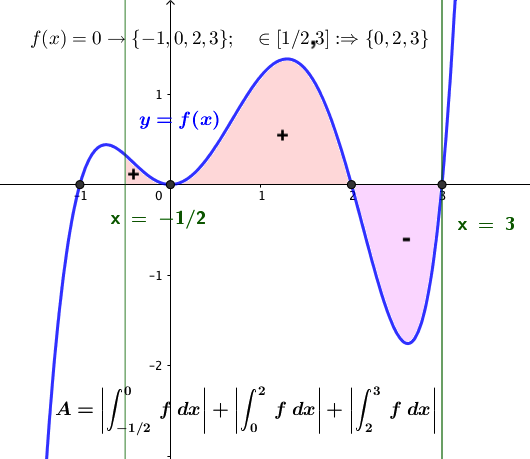
\includegraphics[width=.75\textwidth]{imagenes/imagenes08/T08IM12.png}
	\end{figure}

ÁREA ENCERRADA ENTRE DOS FUNCIONES $f$ y $g$ en $[a,b]$:

\hspace{5 mm} (1) En esta ocasión, buscamos los puntos de corte entre funciones, `nodos' en $[a,b]$, es decir buscamos las soluciones de la ecuación $f(x)=g(x)$, supongamos que estas soluciones son  $\left\{x_1<x_2< \cdots <x_n\right\} \in  [a,b]$. entonces el área es:

\hspace{5 mm} (2) Área = $\; \displaystyle \left| \int_a^{x_1} (f(x)-g(x)) \; \dd x \right| + \left| \int_{x_1}^{x_2} (f(x)-g(x)) \; \dd x \right| + \cdots + \left| \int_{x_n}^b (f(x)-g(x)) \; \dd x \right| $

Si no se especifica el intervalo de integración, el área será las sumas de los valores absolutos de la integral definida desde un `nodo' hasta el siguiente de la función $(f-g)$.

	\begin{figure}[H]
 		\centering
		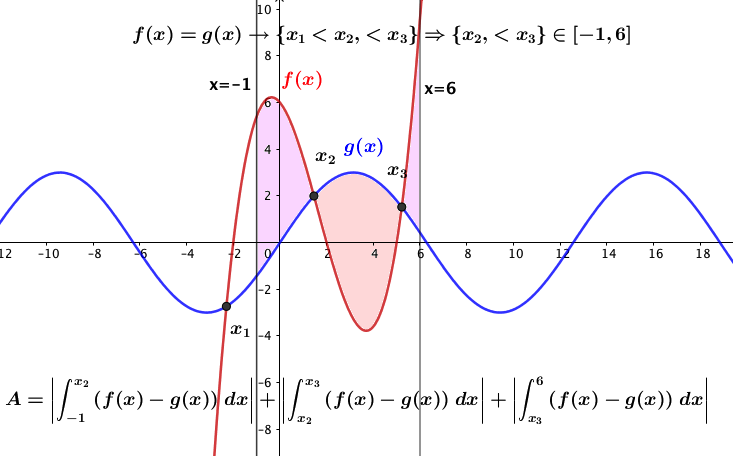
\includegraphics[width=.75
		\textwidth]{imagenes/imagenes08/T08IM13.png}
	\end{figure}

ÁREA LIMITADA POR UNA CURVA CERRADA:
\begin{multicols}{2}
La curva cerrada vendrá, generalmente, dada por una función implícita $F(x,y)=0$, de la que debemos obtener $f_1$ y $f_2$ despejando la $y$.

\vspace{5mm} Área = $\displaystyle \left| \; \int_a^b (f_1(x)-f_2(x))\; \dd x \; \right|$

	\begin{figure}[H]
 		\centering
		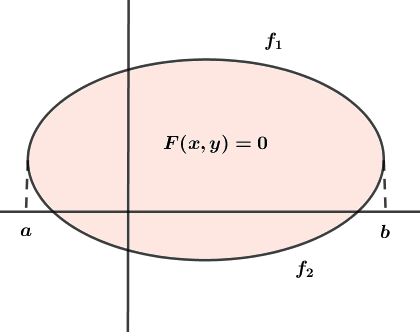
\includegraphics[width=.4\textwidth]{imagenes/imagenes08/T08IM14.png}
	\end{figure}
\end{multicols}

\begin{ejem}
Calcula el área encerrada por $y=f(x)=x^3-6x^2+8x$ con el eje $OX$.	

(1) $\quad f(x)=x^3-6x^2+8=x(x-2)(x-4)0 \; \to \;   x=0\; x=2; x=4$

(2) Como no nos limitan a integrar en ningún intervalo, lo haremos desde $0$ hasta $2$ y, desde ahí hasta $4$

\begin{multicols}{2}
Área = $\; \displaystyle \left| \int_0^2 (x^3-6x^2+8x)\; \dd x  \right| +  \left| \int_2^4 (x^3-6x^2+8x)\; \dd x  \right| =\left|\;  \eval[\dfrac {x^4}{4}-2 x^3+4x^2|_0^2 \; \right| + \left|\;  \eval[\dfrac {x^4}{4}-2 x^3+4x^2|_2^4 \; \right| = \left| (4-16+16)-(0) \right| + \left| (64-128+64)-(4-16+16) \right|= |4|+|-4|=8 u^2$


\begin{figure}[H]
 		\centering
		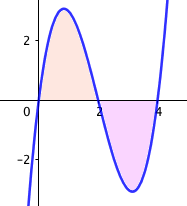
\includegraphics[width=.25\textwidth]{imagenes/imagenes08/T08IM15.png}
	\end{figure}
\end{multicols}

!`Usamos $u^2\;$ para referirnos a unidades de área (siendo $u\;$ la unidad arbitraria de longitud!

\textcolor{gris}{Compruebe el lector que $\displaystyle \int_0^4 (x^3-6x^2+8x)\; \dd x =0$. Obvio, como $f$ no es positiva en $[0,4]$, la integral no representa el área. }
\end{ejem}

\begin{ejem}
Calcula el área entre las funciones $f(x)=\sin x$ y $g(x)=\cos x$, en $[\pi/4, 7\pi/4]$.	


(1) Busquemos, primero, los `nodos', puntos de corte de $f$ con $g$:

$f(x)=g(x)\to \sin x = \cos x \to \tan x= \pi/4+k\;\pi; \quad \forall k\in \mathbb Z$

En el intervalo considerado: $[\pi/4, 7\pi/4] \to f=g \leftrightarrow x_1=5\pi/4   $

(2) La integral buscada será A = $\displaystyle \left| \int_{\pi/4}^{5\pi/4} (\sin x - \cos x)\; \dd x  \right| +  \left| \int_{5\pi/4}^{7\pi/4} (\sin x - \cos x)\; \dd x  \right|  = \eval[-\cos x - \sin x|_{\pi/4}^{5\pi/4}+ \eval[-\cos x - \sin x|_{5\pi/4}^{7\pi/4}=
\left| (\sqrt{2}/2)+(\sqrt{2}/2) \right| +$$+ \left| (-\sqrt{2}/2+\sqrt{2}/2)-(\sqrt{2}/2+\sqrt{2}/2) \right|=
|2\sqrt{2}|+|-\sqrt{2}|=3\sqrt{2} $

Adjuntamos una imagen para aclarar el área que hemos calculado:
\begin{figure}[H]
 		\centering
		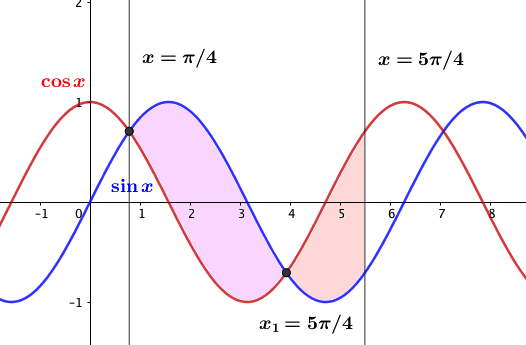
\includegraphics[width=.8
		\textwidth]{imagenes/imagenes08/T08IM16.png}
	\end{figure}

\end{ejem}

\begin{ejem}
Calcula el área de la elipse: $\dfrac{x^2}{16} + \dfrac {y^2}{9} =1$	

\textcolor{gris}{Es sabido que el área de una elipse, de semiejes $a$ y $b$ es $\pi\; a\: b$, como la ecuación de una elipse (centrada en el origen) de semiejes $a$ y $b$ es $\dfrac{x^2}{a^2}+\dfrac{y^2}{b^2}=1$, luego como resultado debemos obtener $A=\pi \; 4\cdot 3 = 12 \pi\; u^2$  }

Despejemos la $y$ de nuestra elipse dada como función implícita: 

$\displaystyle y^2=9\cdot \left(1-x^2/16 \right)=\frac 9 {16} \cdot (16-x^2) \to \begin{cases}
 f_1=+\frac 3 4 \sqrt{16-x^2}	\\
 f_2=-\frac 3 4 \sqrt{16-x^2}
 \end{cases}$
 
 Busquemos los límites de integración, cuando cortan al eje $OX \equiv y=0$:
 
$\dfrac{x^2}{16} + \dfrac {y^2}{9} =1 \to y=0 \Rightarrow \dfrac{x^2}{16}  =1 \to x^2=16 \to x_1=-4; \; x_2=+4 $ 

Por lo que Área= $\displaystyle \left| \int_{x_1}^{x_2}(f_1-f_2)\; \dd x \right|= \left| \int_{-4}^{4} \left( 2\;\frac 3 4 \sqrt{16-x^2} \right) \; \dd x \right|= \frac 3 2 \left| \int_{-4}^{4} \sqrt{16-x^2} \; \dd x \right|$

Busquemos una primitiva, pues esta integral necesita un CV, pues se trata de una integral irracional algebraica de cambio trigonométrico: $x=4 \sin t; \quad \dd x= 4 \cos t \; \dd t$

$\displaystyle \int \sqrt{16-(4 \sin t^2}); \cos r\; \dd t = 4 \int \cos^2 t\; \dd t = \; \to$ (fórmulas de reducción) = $\displaystyle 4 \int \frac 1 2 (1+\cos 2t)\; \dd t= 2 (t+\frac 1 2 \sin 2t)= 2t + 2 \sin t \cos t = \; \to$ (Deshacer CV) 

$\to \; = \displaystyle 2\arcsin \frac x 4 + 2 \frac x 4 \cdot  \sqrt{1-\frac {x^2}{16}}+\mathcal C= \frac 1 4\; x\sqrt{16-x^2}+2\arcsin \frac x 4 + \mathcal C$ 

Luego, Área= $\frac 3 2 \left| \int_{-4}^{4} \sqrt{16-x^2} \; \dd x \right| = \eval[\frac 3 8 x \sqrt{16-x^2}+3 \arcsin {(x/4)}|_{-4}^4= \cdots= 12\pi$

Adjuntamos, también,  una imagen para aclarar el área que hemos calculado:
\begin{figure}[H]
 		\centering
		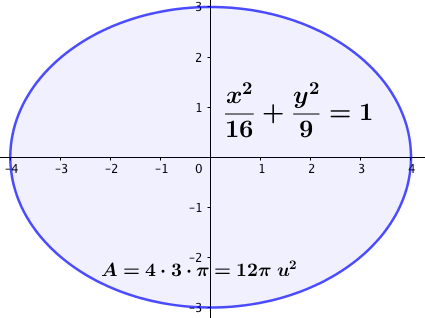
\includegraphics[width=.45
		\textwidth]{imagenes/imagenes08/T08IM17.png}
	\end{figure}
\end{ejem}
\subsubsection{\underline{Ejercicios resueltos de áreas de figuras planas}}
%$A=\displaystyle \left| \int_{a}^{b} f \: \dd x \right|$
\begin{ejre}
Calcula el área encerrada con $OX$ por las funciones:

\begin{multicols}{2}
\begin{enumerate}[a) ]
\item $f(x)=\cos x$, en $[\pi/2,2\pi]$
\item $f(x)=x^2-x-2$
\item $f(x)=x^3-x^2-6x$
\item $y=\sqrt{x}$,  entre $x=0\; $ y $\; x=4$
\item $f(x)=(x^2-x)\; e^x$
\item $f(x)=\sin x$ y las rectas $x=0$ y $x=2\pi$
\end{enumerate}	
\end{multicols}

\end{ejre}

\begin{proofw}\renewcommand{\qedsymbol}{$\diamond$}


\hspace{5mm} $a) \qquad $ Busquemos donde $f(x)$ corta al eje $OX$ en 	$[\pi/2, 2\pi]$: 

$\cos x = 0 \to x=\pi/2+k\pi; \; \forall k \in \mathbb Z \Rightarrow $, en el intervalo considerado: $x_1=3\pi/2$

Luego, el área pedida será: 

A=$\displaystyle \left| \int_{\pi/2}^{3\pi/2} \cos x \; \dd x \right| + \left| \int_{3\pi/2}^{2\pi} \cos x \; \dd x \right|= 
\left| \eval[\sin x|_{\pi/2}^{3\pi/2} \right| +\left| \eval[\sin x|_{3\pi/2}^{2\pi} \right|=$

$=\displaystyle \left| (-1)-(-1) \right| + \left| (0)-(-1) \right|=|-2|+|1|=3 \; u^2$

\vspace{2mm}$b) \qquad$ Ahora no nos dan límites de integración (intervalo donde calcular el área). El área será la suma de todos los valores absolutos de las ID de $f$ de corte a corte con $OX$ (ordenados).
$\; x^2-x-2=0=(x-2)(x+1) \to x=-1 \; \wedge \; x=2\; $. Por lo que:

$A=\displaystyle \left| \int_{-1}^2 (x^2-x-2)\; \dd x \right|= \eval[\dfrac {x^3}{3}-\dfrac {x^2}{2}-2x|_{-1}^2= \left|\;  (8/3 -2-4)-(-1/3-1/2+2)\;  \right|=|-9/2|= 9/2 \; u^2$

\vspace{2mm}$c) \qquad$ Puesto que no tenemos límites de integración determinado, integraremos de corte a corte.
$\; x^3-x^2-6x=0 \Rightarrow x=\{-2, 0, 3\} \; $. El área será:

$A=\displaystyle \left| \int_{-2}^{0} (x^3-x^2-6x) \: \dd x \right|+ \left| \int_{0}^{3} (x^3-x^2-6x) \: \dd x \right| = \left| \eval[x^4/4-x^3/3-3x^2|_{-2}^0   \right| + \left| \int_{0}^{3} (x^3-x^2-6x) \: \dd x \right|= |16/3|+|-63/4|=253/12\; u^2$

\vspace{2mm}$d) \qquad$ Como $\sqrt{x}=0$ no tine soluciones en $]0,4[$. El área pedida es:

$A=\displaystyle \left| \int_{0}^{4} x^{1/2} \: \dd x \right|=\eval[\frac {2}{3}\; \sqrt{x^3}|_0^4= \frac 2 3 \left| ( 8)-(0)  \right|= 16/3\; u^2$

\vspace{2mm}$e) \qquad$ Como no nos dan los límites de integración, buscamos los cortes con $OX:\; y=0$ e integraremos de corte a corte.

$(x^2-x)\; e^x=0; \quad$ como $e^x>0, \; \forall x \in \mathrm{R} \to x^2-x=x(x-1)=0 \Rightarrow x=0\; \wedge \; x=1 $

$A=\displaystyle \left| \int_0^1 (x^2-x)\; e^x \;\dd x  \right|=$
$(\text{ PARTES, dos veces})= $
$\eval[e^x\; (x^2-3x+3)|_0^1=|e-3| = (3-e)\; u^2$

\vspace{2mm}$f) \qquad$ Hemos de calcular el área encerrada por $y=\sin x$ con $OX$ en $[0,2\pi]$, busquemos donde corta al eje $X$ la función \emph{seno} en  $[0,2\pi]$:
$\sin x = 0 \to x=+k\pi, \; \forall K\in \mathbb R$. En $[0,2\pi]$, $\sin x =0\; $ en $\; x=\pi \; $ 

$A=\displaystyle  \left| \int_{0}^{\pi} \sin x \; \dd x \right| + \left| \int_{\pi}^{2\pi} \sin x \; \dd x \right| $
$\displaystyle \left| \; \eval[-\cos x|_{0}^{\pi} \; \right| \; +\;   \left| \; \eval[-\cos x|_{\pi}^{2\pi} \; \right| =$

$= |\; (1)-(-1)\; | \; +\; |\; (-1)-(1)\; | = |2|+|-2|=4\; u^2 $

\end{proofw}

\emph{Nótese que, realmente, calcular el área encerrada por $f(x)$ con $OX$ se puede considerar como el área encerrada entre dos funciones: $f(x)$ y $g(x)=y=0$, que es la ecuación del eje $OX$.}


\vspace{2mm}

\begin{ejre}
Calcula el área encerrada ente las funciones siguientes:

\begin{multicols}{2}
\begin{enumerate}[a) ]
\item $f(x)= x\; $ y $\; g(x)=x^2$
\item $f(x)=-x^2+6x\; $ y $\; g(x)=x^2-2x$ y las rectas $x=0$ y $x=2$
\item $y=x^4+x^3\; $ e $\; y=x^4+x^2+6x$
\item $y=x^2-5\;$ e $\; y=-x^2+5$
\item $y=x^3+8x$ con $y=6x^2$
\end{enumerate}	
\end{multicols}
\end{ejre}

\begin{proofw}\renewcommand{\qedsymbol}{$\diamond$}


\hspace{5mm} $a) \qquad $ Como no nos dan límites de integración, integraremos de `nodo' a `nodo' $\to f(x)=g(x)\to x=x^2\to x^2-x=0 \to x(x-1)=0 \Rightarrow x=0\; \wedge \; x=1$

$A=\displaystyle \left| \int_{0}^{1} (f-g) \: \dd x \right|\left| = \int_{0}^{1} (x^2-x) \: \dd x \right|= \; \to \;$ 
[\footnotesize{ da igual tomar $f-g$ que $g-f$, tomamos, después, valor absoluto } \normalsize{]}
$\displaystyle \; \to\; = \left| \eval[x^3/3-x^2/2|_0^1 \right|= |(1/3-1/2)-(0)|=|\; -1/6 \;|= 1/6 \; u^2$



\vspace{2mm}$b) \qquad$ Busquemos primero los nodos de $f$ y $g\;$, en el intervalo $[0,2]$: $f(x)=g(x) \to -x^2+6x=x^2-2x \to 2x^2-8x=0 \to 2x(x-4)=0 \rightarrow x=0 \; \wedge \; x=4\; $, en  $]0,2[\; $ no tenemos ningún nodo. Integraremos pues, $f-g$ desde $x=0$ hasta $x=2$

$A=\displaystyle \left| \int_{0}^{2} (2x^2-8x) \: \dd x \right| = \eval[2x^3/3-4x^2|_0^2 = \left| (16/3-16)-(0) \right|=|-32/3|=32/3 \; u^2 $

\vspace{2mm}$c) \qquad$ Como no tenemos límites de integración, buscaremos los nodos (puntos de corte entre las dos funciones) e integraremos de nodo a nodo. Llamaremos $f$ a la primera de las funciones y $g$ a la segunda.

$f=g\to x^4+x^3=x^4+x^2+6x \to (f-g):\; x^3-x^2-6x=0 \Rightarrow  x=\{-2, 0, 3\}$
El problema es el mismo que el del apartado $c$ del ejercicio anterior, sumar los valores absolutos de las integrales de $f-g=x^3-x^2-6x$, desde $-2$ hasta $0$ y desde $o$ hasta $3$. Por tanto: $A=253/12\; u^2$-

\vspace{2mm}$d) \qquad$ Como en el apartado anterior, no tenemos límites de integración, buscaremos los nodos (puntos de corte entre las dos funciones) e integraremos de nodo a nodo. Llamaremos $f$ a la primera de las funciones y $g$ a la segunda.



$f=g\to x^2-5=-x^2+5 \to \; (f-g)=\; 2x^2-10=0 \Rightarrow x=\pm \sqrt{5}$

$A=\displaystyle \left| \int_{-\sqrt{5}}^{\sqrt{5}} (2x^2-10) \: \dd x \right|= \eval[2x^3/3-10x|_{-\sqrt{5}}^{\sqrt{5}}=\cdots=\frac {40}{3}\sqrt{5}\; u^2$

\vspace{2mm}$e) \qquad$  Llamaremos $f_1$ a la primera función y $f_2$ a la segunda y buscaremos los cortes entre ellas: : $f_i=f_2 \to x^3+8x=6x^2 \to x^3-6x^2+8x=0 \to x(x^2-6x+8)=x(x-2)(x-4)=0 \Rightarrow x=\left\{ 0, 2 , 4 \right\}$

$A=\displaystyle \left| \int_{0}^{2} (x^3-6x^2+8x)\;  \dd x \right| + 
\left| \int_{2}^{4 } (x^3-6x^2+8x) \; \dd x \right| =
\eval[x^4/4-2x^3+4x^2|_0^2 +$

$+ \eval[x^4/4-2x^3+4x^2|_2^4 =
\left| (4-16+16)-(0) \right| + \left| (64-128+64)-(4-16+16) \right|=$ 

$=|4|+|-4|= 8\; u^2$

 
\end{proofw}

\emph{Para calcular el área encerrada entre tres funciones, se hace preciso un dibujo que nos aclare el recinto cuya área queremos calcular.}

\begin{ejre}
Calcula el área del plano limitado por la parábola $y^2-x=1$ y por la recta paralela a $y=x$	que pasa por el punto $(-1,0)$
\end{ejre}

\begin{proofw}\renewcommand{\qedsymbol}{$\diamond$}

La primera función viene dada en forma implícita, hay que despejar $y$ con lo que aparecerán dos funciones: $\; f_1(x)=+\sqrt{x+1}\;$ y $\; f_2(x)=-\sqrt{x+1}\;$ 

Por otra parte, las rectas paralelas a $y=x$ son de la forma $y=x+k$, para que pase por $(-1,0)$ la función (recta) será $g(x)=y=x-1$

Hay que buscar el área encerrada por tres curvas. Se hace necesaria una gráfica de las mismas que nos aclare qué es  lo que debemos integrar. (las funciones son sencillísimas de dibujar).

$f= g \to \pm \sqrt{x+1}=x-1 \Rightarrow x=-1 \; \wedge \; x=3$ 

Desde $-1$ hasta $0$, las funciones que encierran área son $f_1$ y $f_2$ y desde $0$ hasta $3$, las funciones que encierran área son $f_1$ y $g$
Así, el área buscada será:

\begin{multicols}{2}
$A=\displaystyle \left| \int_{-1}^{0} (f_1-f_2) \: \dd x \right| + \left| \int_{0}^{3} (f_1-g) \: \dd x \right|= \left| \int_{-1}^{0} (2\sqrt{x+1}) \: \dd x \right| + \left| \int_{0}^{3} (\sqrt{x+1}-x+1) \: \dd x \right|=
\eval [\dfrac {4}{3}\sqrt{(x+1)^3}|_{-1}^0 + \eval[\dfrac 2 3 \sqrt{(x+1)^3}-\dfrac {x^2}{2}+x|_0^3=
\left| \left(\dfrac 4 3\right)-(0)\right|+ \left| \left(\dfrac 2 3 \cdot 2^3 - \dfrac 9 2 + 3\right)-\left(\dfrac 2 3 \right)\right|=
\dfrac 4 3 + \dfrac {19}{6}= \dfrac 9 2 \; u^2$

\begin{figure}[H]
 		\centering
		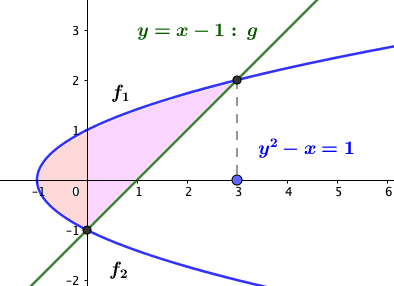
\includegraphics[width=.45
		\textwidth]{imagenes/imagenes08/T08IM18.png}
	\end{figure}	
\end{multicols}
	
\end{proofw}

\begin{ejre}
Calcula el área del plano limitado por la curva $f(x)=+\sqrt{\dfrac {x}{2}}$ y por la función $g(x)=|x-1|$.
\end{ejre}

\begin{proofw}\renewcommand{\qedsymbol}{$\diamond$}

Ahora la que realmente son dos funciones es la $g$ que es definida a trozos: 

$g(x)=\begin{cases}
1-x = g_1(x)& \text{ si } x\le 1 \\
x-1 = g_2(x)& \text{ si }  x>1	
\end{cases}\; $ 

Hace falta un dibujo para ver el recinto del que queremos calcular el área.

\begin{figure}[H]
 		\centering
		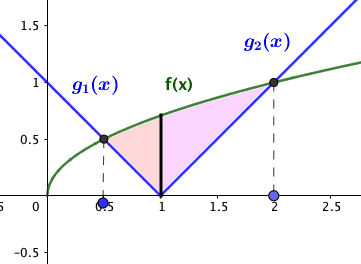
\includegraphics[width=.50
		\textwidth]{imagenes/imagenes08/T08IM19.png}
\end{figure}
$f=g\to (\sqrt{x/2})^2=|x-1|^2 \to $
$x/2=x^2-2x+1 \rightarrow x=1/2 \; \wedge \; x=2 $ 



Se observa de la figura que hemos de integrar, desde $1/2$ hasta $1$ la función $f-g_1$ y desde $1$ hasta $2$ la función $f-g_2\;$.


$A=\displaystyle \left| \int_{1/2}^{1} \left(\sqrt{\dfrac x 2}-(1-x)  \right) \: \dd x \right|+  \left| \int_{1}^{3} \left(\sqrt{\dfrac x 2}-(x-1)  \right) \: \dd x \right|=$

$\displaystyle =\left| \int_{1/2}^{1} \left(\sqrt{\dfrac x 2}+x-1  \right) \: \dd x \right|+  \left| \int_{1}^{3} \left(\sqrt{\dfrac x 2}-x+1  \right) \: \dd x \right|=$

$\displaystyle = \left| \eval[\dfrac 4 3 \sqrt{\left( \dfrac x 2 \right)^3}+\dfrac {x^2}{2}-x|_{1/2}^{1} \right| + \left| \eval[\dfrac 4 3 \sqrt{\left( \dfrac x 2 \right)^3}-\dfrac {x^2}{2}+x|_{1}^{3} \right|=\cdots = 13/24 \; u^2$
\end{proofw}

\begin{ejre}
Encuentra el polinomio de segundo grado tal que pasa por los puntos $(0,1)\;$ y $\;(3,0)$, sabiendo que el área encerrado por ese polinomio con $OX$ en $[0,3]$ es 4	
\end{ejre}

\begin{proofw}\renewcommand{\qedsymbol}{$\diamond$}

Como $p(x)$ pasa por $(3,0)$, $3$ es una raíz de $p(x)=(x-3)(ax+b)$

Como $p(x)$ pasa por $(1,0):\to x=1 \leftrightarrow y=0 \Rightarrow b=-1/3$

Luego $p(x)=(x-3)(ax-1/3)$

$p(x)=0 \leftrightarrow x=3 \; \vee \; x=1/{3a}$ (*) Supongamos $1/{3a} \notin [0,3]$, entonces, el área es:

$A=\displaystyle \int_0^3 (x-3)(ax-1/3)\; \dd x = =\eval[-3ax^2/2-x^2/6+x|_0^3= $

$=9a-27/2\; a-3/3+3 = 4/3 \to a=1/27$

Luego el polinomio es $y=(x-3)(x/27 - 1/3)$

\textcolor{gris}{Los ceros de $p(x)$ son $3$ y $9$, luego la suposición (*) es correcta ($9 \notin [0,3]$).}
	
\end{proofw}

\begin{ejre}
Se consideran las curvas $y=x^2\; $ e $\; y=a$, con $0<a<1$. Ambas curvas se cortan en el punto $(x_0,y_0)$, con la abcisa positiva. Encuéntrese $a$ sabiendo que el área encerrada entre ambas curvas desde $x=0$ hasta $x=x_0$ es la misma que la encerrada entre $x=x_0$ y $x=1$	
	
\end{ejre}


\begin{proofw}\renewcommand{\qedsymbol}{$\diamond$}


\begin{multicols}{2}

Punto de corte de ambas curvas:

$(x_0,y_0) \to x^2= a \to x=\pm\sqrt{a}$,
siendo la abacisa del punto de corte positiva, 
$x=+\sqrt{a}  $ y el punto de corte será:
$(\sqrt{a}, a)$

Integraremos desde $0$ hasta $\sqrt a$  la función $f$ y desde $\sqrt a$ hasta $1$ la función $(f-g)$, luego tomaremos valores absolutos.
	\begin{figure}[H]
	\centering
	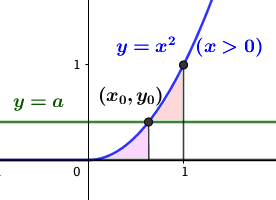
\includegraphics[width=.45\textwidth]{imagenes/imagenes08/T08IM20.png}
	\end{figure}
\end{multicols}

$A_1=\displaystyle \left| \int_{0}^{\sqrt{a}} x^2 \; \dd x \right| \; ; \; A_2 = \left| \int_{\sqrt{a}}^{1} (x^2-a) \; \dd x \right| \Rightarrow $

$ A_1=\left| \; \eval[x^3/3|_{0}^{\sqrt{a}} \; \right|\; ; \; A_2=\left| \; \eval[x^3/3+ax|_{\sqrt{a}}^{1} \; \right| \Rightarrow$

$ A=1=\left| \left(\dfrac{2a\sqrt{a}}{3} \right)-(0) \right| \; ; \; A_2= \left| \left(\dfrac 1 3 - a+ \dfrac {2a\sqrt{a}}{3} \right) \right|\Rightarrow$

Simplificando e igualando las áreas $\dfrac {2a\sqrt{a}}{3}= \dfrac 1 3 -a + \dfrac {2a\sqrt{a}}{3} \Rightarrow a=\dfrac 1 3 $

\end{proofw}


%$A=\displaystyle \left| \int_{a}^{b} f \: \dd x \right|$
\subsubsection{\underline{Ejercicios propuestos de áreas de figuras planas}}

\begin{enumerate}
	
\item Calcula las áreas de las siguientes áreas: 
	\begin{enumerate}[a) ]
	\item $y=3x^2-x+1$, el eje $OX$ y las rectas $x=0\; $ y $\; x=4$ 
	\item $y=x^3-3x^2+3x\; $ y $\; y=x$
	\item $y=x(x-1)(x-2)\;$ y $\; y=0$
	\item $y=x^2\;$ y $\; y=1$
	\end{enumerate}

\rightline{\textcolor{gris}{Solución: $a)\quad 60\;u^2; \qquad b) \quad 1/2\; u^2; \qquad c) 	\quad 1/2\; u^2; \; \qquad d) \quad 4/3 \; u^2$}}

\item Halla el área limitada por la función $y=2x-x^2$ y sus tangentes en los puntos en que corta al eje de abcisas.

\rightline{\textcolor{gris}{\tiny{Solución: Como es la gráfica entre tres funciones, conviene una representación gráfica 8es sencilla)}. Área= $2/3\; u^2$}}

\item Dibuja el recinto comprendido entre las gráficas $y=\dfrac 1 {x^2}\; $; $\; y=x\;$ y $\; y=8x\; $ y calcula el área del recinto que encierran entre las tres funciones.

\rightline{\textcolor{gris}{Solución: $3/2 \; u^2$ }}

\item Dada la función $f(x)=ax^3+bx^2+cx+d\;$, se sabe que tiene un máximo relativo en $x=1\; $, un punto de inflexión en el origen de coordenadas y que $\displaystyle \int_0^1 f(x)\; \dd x = \dfrac 5 4 $. Calcula $a$, $b$, $c$ y $d$.

\rightline{\textcolor{gris}{Solución: $d=0; \; b=0; \; a=-1; \; c=3  \; \to \;  f(x)=-x^3+3x$ }}	

\item Calcula el área comprendida entre las funciones $y=e^x\; $ y $\; y=2x-x^2\;$ y las rectas $x=0$ y $x=2$.

\rightline{\textcolor{gris}{Solución: $(e^2-7/3)\; u^2$ }}

\item Calcula el valor de $b>0$ sabiendo que el área encerrada por las funciones $y=x^2\;$ y $\; y=bx$ es igual a $\dfrac 9 2 \; u^2$.

\rightline{\textcolor{gris}{Solución: $b=3$ }}

\item Considera la región del plano comprendida por las curvas $y=e^x\;$ y $\; y=e^{2x}\; $ y la recta vertical $x=k$

\hspace{10mm}$a)\; \; $Halla el área para $k=1$.

\hspace{10mm}$b)\; \;$ Determina el valor de $k>0$ para que el área sea 2.

\rightline{\textcolor{gris}{Solución: $a) \quad (e^2/2-e+1/2)\; u^2;  \qquad b) \quad k=\mathrm{ln} \; 3$}}

\item Calcula el área de la elipse $\; \dfrac{x^2}{a^2}+\dfrac{y^2}{b^2}=1 \;$

\rightline{\textcolor{gris}{Solución: $A=\pi\; a \; b$}}

\item Calcula el área de cada una de las regiones limitadas por la parábola $y=x^2\; $ y la circunferencia $\; x^2+yY2=2$.

\rightline{\textcolor{gris}{Solución: $a) \quad \pi/2+2/3; \qquad b) \quad 3\pi/2-2/3$}}

\item Calcúlese el área del menor de los recintos limitados por la circunferencia $x^2+y^2=5\; $ y la hipérbola $\; x\; y = 2$. 

\rightline{\textcolor{gris}{Solución: $\arcsin \; \dfrac 2 {\sqrt{5}}- \arcsin \; \dfrac 1 {\sqrt{5}}+ 2 \mathrm{ln}\; 2$}}
\end{enumerate}

%$A=\displaystyle \left| \int_{a}^{b} f \: \dd x \right|$

\subsection{Cálculo de un arco de curva $\; \divideontimes $}

		


\underline{Curvas en forma explícita}: $y=f(x)$

Si $f$ tiene derivada continua en $[a,b]$ (Curva $\Gamma$ \emph{rectificable}), su longitud vale:

\hspace{20mm} $\boxed{\; \displaystyle l(\Gamma)=\int_a^b \sqrt{1\; + \; (f'(x))^2}\; \dd x\; }$

	\begin{figure}[H]
	\centering
	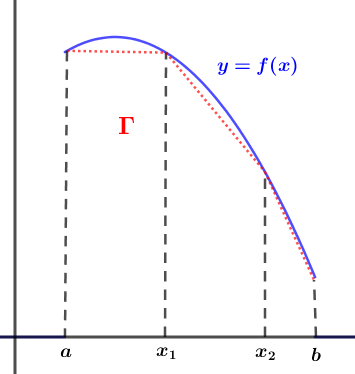
\includegraphics[width=.45\textwidth]{imagenes/imagenes08/T08IM21.png}
	\end{figure}

\underline{Curvas en forma paramétrica}: (*)$\begin{cases}
x=x(t) \\ y=y(t) \end{cases} \quad a\le t \le b$

\vspace{2mm}

\textcolor{gris}{El concepto de curva plana es más general que el de gráfica de una función. Una \textbf{curva plana} es un conjunto de puntos de la forma $(\; x(t)\; ,\; y(t)\; )$, siendo $x(t)\; e $\; $y(t)$ dos funciones reales continuas en $[a,b]$.}

\textcolor{gris}{$w:[a,b] \to \mathbb R^2 \; / \; t  \leadsto (\; x(t)\; ,\; y(t)\; ) $ se dice que es una \textbf{parametrización} de la curva.  Las ecuaciones (*) son las \textbf{ecuaciones paramétricas de la curva}  }

\textcolor{gris}{Si $w(a)=w(b)\to $ tenemos una \textbf{curva cerrada}; si $w$ es inyectiva tenemos una \textbf{curva simple}.  Ejemplo: Para $t\in [0,2\pi], la curva \begin{cases} x=\cos t \\ y = \sin t \end{cases}$ es una `circunferencia' (simple y cerrada).}

\vspace{2mm}

Si existen y son continuas $x'(t)\; $ e $\; y'(t)$ en $[a,b]$ la curva es rectificable y su longitud es:

\hspace{20mm} $\boxed{\;\displaystyle l(\Gamma)=\int_a^b \sqrt{x'(t)^2 + y'(t)^2}\; \dd t\; }$

\vspace{5mm}

\emph{Normalmente, el cálculo de longitudes de arcos de curvas lleva a integrales muy complicadas.} Veremos algunos ejemplos más sencillos.

\vspace{3mm}

\begin{ejem}
$\divideontimes \; $Calcúlese la longitud del `astroide' $x^{2/3}+y^{2/3}=a^{2/3}$


	

Al despejar $y$ de esta función implícita, tenemos dos funciones:

\hspace{15mm} $f_1(x)=y_1=+\sqrt{(\; a^{2/3}-x^{2/3}\; )^3}$

\hspace{15mm} $f_2(x)=y_2=-\sqrt{(\; a^{2/3}-x^{2/3}\; )^3}$

Ambas definidas y simétricas en $[-a,a]$

\begin{multicols}{2}
\begin{figure}[H]
	\centering
	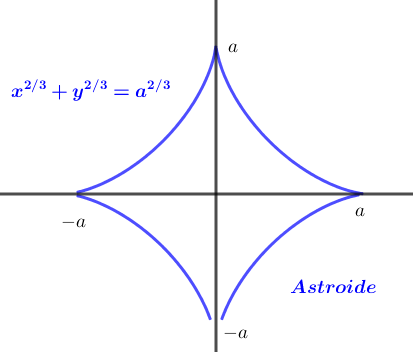
\includegraphics[width=.4\textwidth]{imagenes/imagenes08/T08IM22.png}
	\end{figure}
Bastará con calcular la longitud de un cuarto de la curva y multiplicar por cuatro. (ver figura adjunta).

$\quad$

$\displaystyle \frac 1 4 l(\Gamma)= \int_0^a \sqrt{1+(y_1')^2} \; \dd x$
\end{multicols}

$y_1'= \frac 3 2 \left( a^{2/3}-x^{2/3} \right)^{1/2}\cdot \left( -\dfrac 2 3 x^{-1/3} \right)= - \sqrt{ \dfrac {a^{2/3}-x^{2/3}}{x^{2/3}}}$

$\displaystyle \frac 1 4 l(\Gamma)= \int_0^a \sqrt{1+ \dfrac {a^{2/3}-x^{2/3}}{x^{2/3}}}\; \dd x =\int_0^a \dfrac {a^{1/3}}{x^{1/3}}\; \dd x = \text { (inmediata) }= \frac 3 2 a$

\hspace{20mm}$\Rightarrow\; \; $ Luego: $\quad \displaystyle  l(\Gamma)=4\cdot \frac 3 2 a= 6\; a\; \; u$  
\end{ejem}

\begin{ejem}
Si la posición de un móvil en el plano viene dada por las ecuaciones $x(t)=t^2$ e $y(t)=t-t^3/3$, donde t representa el tiempo, entonces, el espacio recorrido en los instantes $0\le t \le 2$ es la longitud del arco definido por esas ecuaciones paramétricas. Calcula, pues, el espacio recorrido por este móvil.

$\displaystyle l\; (\Gamma)=\int_a^b \sqrt{x'(t)^2 + y'(t)^2}\; \dd t\;=\; \to \left[ \; x'(t)=2t; \; y'(t)=1-t^2 \; \right]\to = \displaystyle l\; (\Gamma)=\int_0^2 \sqrt{(2t)^2 + (1-t^2)^2}\; \dd x\;= \int_0^2 \sqrt{t^4+2t^2+1} \; \dd t \; = \int_0^2 \sqrt {(t^2+1)^2}\; \dd t = $ 

$=\displaystyle \int_0^1 (t^2+1)\; \dd t= \eval[t^3/3+t|_0^1=(8/3+2)-(0)=14/3 \; u$ 
	
\end{ejem}

\begin{ejem}
Determina la longitud de la curva de ecuación $f(x)= \displaystyle \int_0^x \sqrt{t+3}\; \dd t$, en $[0,1]$

\vspace{2mm}

Como $f'(x)= \left( \displaystyle \int_0^x \sqrt{t+3}\; \dd t  \right)' =\sqrt{x+3}\;$ 	 y  $\; \displaystyle l\; (\Gamma)=\int_a^b \sqrt{1\; + \; (f'(x))^2}\; \dd x\;$, tenemos:

$\displaystyle l\; (\Gamma)= \int_0^1 \sqrt{ 1 + (\sqrt{x+3})^2 } \; \dd x = \int_0^1\sqrt{x+4}\; \dd x= (\text { inmediata })= \eval[\dfrac {2\sqrt{(x+4)^3}}{3}|_0^1= \left(\dfrac {2 \sqrt{5^3}}{2}  \right )-\left( \dfrac {2\; 2^3}{3} \right)= \left(\dfrac{10\sqrt{5}}{3}-\dfrac{16}{3} \right)\; u$

\end{ejem}

\begin{ejem}
Determina la longitud de la curva $w$, en $[0,\pi]$ dada por sus ecuaciones paramétricas: $w\; :\; \begin{cases} x(t)=4\sin t \\ y(t)=4\cos t - 5 \end{cases}$

\vspace{2mm}

$x'(t)=4\cos t; \quad y'(t)= -4\sin t$. Además: $\displaystyle l\; (\Gamma)=\int_a^b \sqrt{x'(t)^2 + y'(t)^2}\; \dd t$

Por lo que:  $\displaystyle l\; (\Gamma)=\int_0^{\pi}
\sqrt{(4 \cos t)^2 + (-4 \sin t)^2}\; \dd t = \int_0^{\pi} \sqrt{16(\sin^2 t + \cos^2 t)}\: \dd t = \int_0^{\pi} 4 \; \dd t= \eval[4t|_0^{\pi}= 4\pi\; u^2 $
	
\end{ejem}


% $\eval[x|_a^b$.   $\eval{x}_0^\infty$

\vspace{4mm}

\subsection{Cálculo de volúmenes de revolución $\; \divideontimes $}

Puesto que dijimos que la ID era una suma de muchos elementos muy pequeños, consideraremos que el volumen engendrado por $f(x)$ al girar $2\pi\;  $ radianes alrededor de $OX$ en $[a,b]$ va a estar formado por infinitos `discos' (cilindros) de radio $f(x)$ y altura $\dd x $, así, el volumen de este disco infinitesimal será $\dd V=\pi\; (f(x))^2\; \dd x$,  y sumando todos los infinitos discos infinitesimales desde $x=a$ hasta $x=b$, tendremos:

\hspace{20mm} $\boxed{ \; \displaystyle V = \; }$
\textcolor{gris}{$\int_a^b \dd V$} 
$\boxed{ \; =\pi\; \int_a^b (f(x))^2\; \dd x\; } $

Si el giro de $2\pi\;  $ radianes se produce alrededor de $OY$, sumando la contribución de infinitos `tubos' infinitesimales, la fórmula se convierte en:

\hspace{20mm} $\boxed{ \; \displaystyle V=2\; \pi\; \int_a^b 
x\cdot |f(x)|\; \dd x \; }$

$\quad$

	\begin{figure}[H]
	\centering
	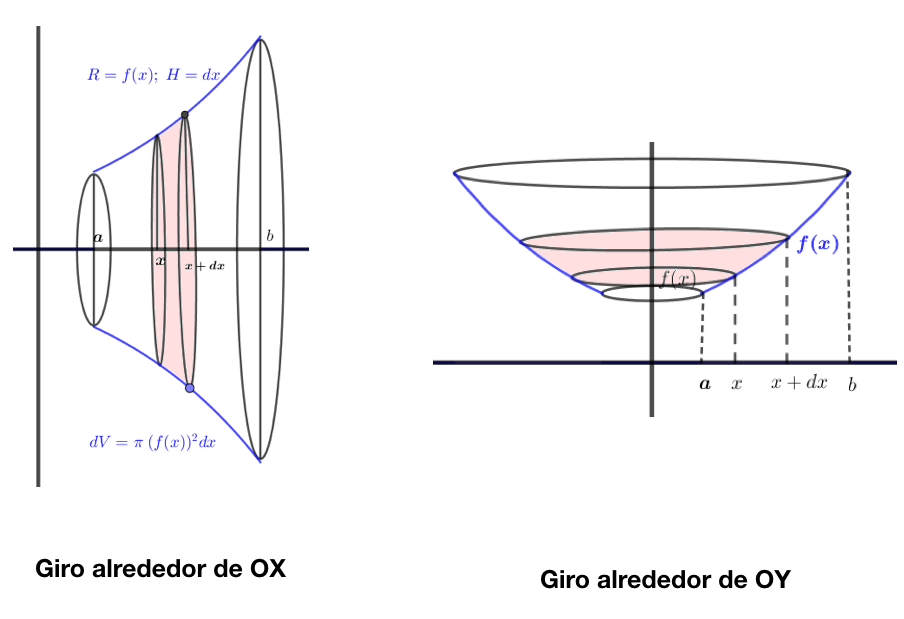
\includegraphics[width=1\textwidth]{imagenes/imagenes08/T08IM23.png}
	\end{figure}

\begin{ejem}
Este ejemplo contempla ambos casos:

\begin{multicols}{2}
	
Considérese la región limitada por la gráfica de la función  $f(x)=x^2-x$ y el eje $OX$. Calcúlese el volumen de revolución del cuerpo engendrado por este recinto al dar un giro completo alrededor de $OX$. Hágase lo mismo para in giro alrededor de $OY$.

\vspace{2mm}

Es fácil obtener una representación gráfica de la figura para hacernos una idea de ambos cuerpos de revoluión (el lector debería poderlos dibujar).
 
	\begin{figure}[H]
	\centering
	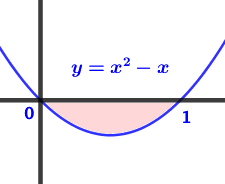
\includegraphics[width=.4\textwidth]{imagenes/imagenes08/T08IM24.png}
	\end{figure}
\end{multicols}
	
$\circ \quad$ \underline{Giro alrededor de $OX$}

$\displaystyle V=\pi\; \int_0^1 (x^2-x)^2\; \dd x = \int_0^1 (x^4-2x^3+x^2)\; \dd x= \eval[x^5/5-x^4/2+x^3/3|_0^1= \pi/30 \; u^3$

$\circ \quad$ \underline{Giro alrededor de $OY$}

Si $x\in[0,1]\to |f(x)|=x-x^2$, con lo que:

$\displaystyle V=2\; \pi\; \int_0^1 x(x-x^2)\; \dd x= 2\; \pi \int_0^1 (x^2-x^3)\; \dd x = \eval [x^3/3-x^4/4|_0^1=\pi/6\; u^3$
	 
\end{ejem}

\subsection{Áreas de superficies de revolución $\; \divideontimes$}
\begin{multicols}{2}
Giro de $2\pi$ alrededor de $OX$ de $f(x)$  en $[a,b]$:

\hspace{10mm} $\boxed{\;\displaystyle A=2\pi\int_a^b f(x)\cdot \sqrt{1+(f'(x))^2}\; \dd x  \;}$



Giro de $2\pi$ alrededor de $OY$ de $f(x)$  en $[a,b]$:

\hspace{10mm} $\boxed{\;\displaystyle A=2\pi\int_{y_1}^{y_2} x(y)\cdot \sqrt{1+(x'(y))^2}\; \dd y  \;}$

	\begin{figure}[H]
	\centering
	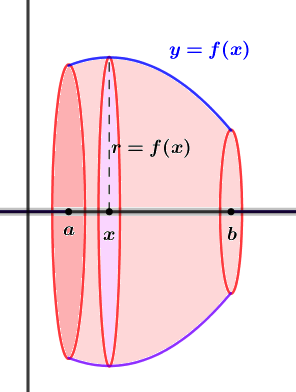
\includegraphics[width=.3\textwidth]{imagenes/imagenes08/T08IM29.png}
	\caption{Giro $OX$}
	\end{figure}
	
\end{multicols}
\begin{ejem}
Demostrar que la superficie de una esfera de radio $R$ es $4\pi R^2$	

\vspace{2mm}

Una esfera la podemos considerar como media circunferencia (la parte positiva) centrada en el origen y de radio $R$ que da un giro completo alrededor de $OX$

$x^2+y^2=R^2 \to y_1=+\sqrt{R^2-x^2}$, luego el área de la esfera será:

$\displaystyle A=2\pi\int_a^b f(x)\cdot \sqrt{1+(f'(x))^2}\; \dd x = 2\pi\int_{-R}^R f_1(x)\; \sqrt{1+(f_1(x))^2}\; \dd x= \; \to $

Si $f_1(x)=+\sqrt{R^2-x^2} \to f'_1(x)= \dfrac {-x}{\sqrt{R^2-x^2}}$, por lo que:

$A=\displaystyle 2\pi\int_{-R}^R \sqrt{R^2-x^2}\dfrac {R}{\sqrt{R^2-x^2}}\; \dd x =\cdots = 2\pi\int_{-R}^R R \dd x= 2\pi \eval [Rx|_{-R}^R= 4\pi R^2 \; u^2$

\emph{Los ejercicios resueltos y propuestos de longitudes de arcos de curvas, volúmenes de revolución y superficies de cuerpos de revolución se incluyen en los ejercicios finales}
\end{ejem}

\begin{figure}[]
	\centering
	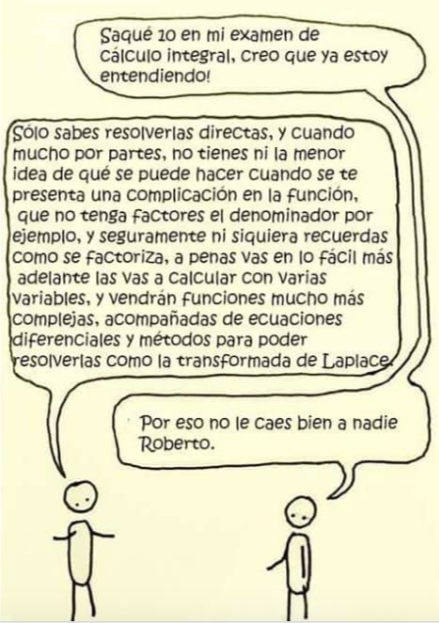
\includegraphics[width=1\textwidth]{imagenes/imagenes08/T08IM25.png}
	\end{figure}

\vspace{6mm}

\section{Ejercicios finales}

\vspace{6mm}

\textbf{\underline{Ejercicios resueltos}}.

\vspace{6mm}

\begin{ejre}
Calcula, usando sumas de Riemann, $\displaystyle	\int_0^3 x^2 \; \dd x $	
\end{ejre}

\begin{proofw}\renewcommand{\qedsymbol}{$\diamond$}	

Como $x^2$ es continua en $[0,3]$, será integrable.

Sea $P_n=0<3/n<2\cdot 3/n<3 \cdot 3/n < \cdots < n\cdot 3/n=n \; ; \quad x_i=3i/n\;\quad x_i-x_{i-1}=3/n \quad f(x_i)= (3i/n)^2 \to \displaystyle \int_0^3 x^2 \; \dd x = \underset {n \to  +\infty}{lim }\; {\sum_{i=0}^{n} } {\left( \dfrac {3i}{n} \right)^2\cdot \dfrac {3}{n}} = \underset {n\to +\infty}{lim}\; { \dfrac {27} {n^3 } \sum_{i=0}^{n} {i^2} } = \; \to $ 

En el capítulo \ref{preliminares} de Preliminares, sección \ref{demostraciones} vimos el `principio de inducción' y en el primer ejemplo (\ref{sum-cuad-induc}), vimos que $\displaystyle \sum_{i=0}^n i^2= \dfrac {n(n+1)(2n+1)}{6}\;$ Usando este resultado:

$\displaystyle \to \; = \underset {n\to +\infty}{lim}\; { \dfrac {27} {n^3} \cdot \dfrac  {n(n+1)(2n+1)}{6} } =
\underset {n \to \infty}{lim}\; {\dfrac {54n^3+\cdots}{6n^3} } = 9$

\textcolor{gris}{Compruebe el/la lector/a el resultado calculando la integral por la regla de Barrow.} 
	
\end{proofw}

\vspace{6mm}

\begin{ejre}
Calcula, gráficamente, las siguientes integrales:

$a)\quad \displaystyle \int_2^4\left( \dfrac x 2 + 1\right)\; \dd x\; ; \qquad \qquad b) \quad \int_{-4}^4 \sqrt{16-x^2}\; \dd x$	
\end{ejre}

\begin{proofw}\renewcommand{\qedsymbol}{$\diamond$}	

Necesitaremos representar las funciones. La primera es una recta y la segunda, $y=+\sqrt{16-x^2}\to x^2+y^2=4^2$, una semi-circunferencia centrada en el origen y radio 4.
$\quad$

$\quad$

$\circ \quad a)$

\begin{multicols}{2}
	\begin{figure}[H]
	\centering
	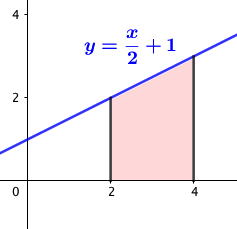
\includegraphics[width=.25\textwidth]{imagenes/imagenes08/T08IM26.png}
	\end{figure}
	\small{La gráfica es un trapecio de bases $2$ y $3$ y altura $2$, Así que}  $A=\dfrac {2+3}{2}\cdot 2=5\; u^2$
\end{multicols}

$\circ \quad b)$

\begin{multicols}{2}

\normalsize{Tenemos una circunferencia de radio $4$,} 

	$\quad $

	$A= \dfrac 1 2 \; \pi \; 4^2= 8 \pi \; u^2$

	\begin{figure}[H]
	\centering
	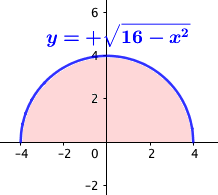
\includegraphics[width=.25\textwidth]{imagenes/imagenes08/T08IM27.png}
	\end{figure}
\end{multicols}
	
\end{proofw}

\begin{ejre}
	Sea $f$ ctna. en $[-1,4]$ y $g(x)=f(x)+2$. Si $\displaystyle \int_{-1}^4 f(x)\; \dd x =5$, Calcula $\displaystyle \int_{-1}^4 g(t)\; \dd t$
\end{ejre}

\begin{proofw}\renewcommand{\qedsymbol}{$\diamond$}		
	$\displaystyle \int_{-1}^4 g(t)\; \dd t = \int_{-1}^4 (f(t)+2)\; \dd t =\int_{-1}^4 f(t)\; \dd t +\int_{-1}^4 2\; \dd t = 5 + \eval[2x|_{-1}^4=
	5+ (8)-(-2)=15$	
\end{proofw}
	



\begin{ejre}
Sea $f(x)=\frac x 3 + 1$, en $[0,3]$	 halla su valor medio en este intervalo y dí el punto de $[0,3]$	donde se alcanza.
\end{ejre}

\begin{proofw}\renewcommand{\qedsymbol}{$\diamond$}	


Como $f$ es ctna en $[0,3]$	, se cumple el th. Valor Medio para integrales.

TVM $f$ en $[0,3]\; $	: $\displaystyle \int_0^3 (\frac x 3 + 1 ) \; \dd x = f(c)\cdot (3-0) $, para algún $c\in [0,3]$	

Gráficamente, si representamos $f>0$ en $[0,3]$	 vemos que se trata de un trapecio de bases $2$ y $1$ y altura $3$, luego su área será $A=\frac {2+1}{2}\cdot 3=9/2=\displaystyle \int_0^3 (\frac x 3 + 1 ) \; \dd x$, al ser $f>0$ y la ID representar el área.

Aplicando TVM del CI: $f(c)\cdot (3-0)=\frac 9 2 \to f(c)=\frac 3 2 = <\;  f \; >$

Como $f(c)=\frac c 3 + 1 = \frac 3 2 \to c=\frac 3 2 \in [0,3]$ 
\end{proofw}


\begin{ejre}
Sin calcular la integral, busca los extremos relativos de la función:
$\; \displaystyle F(x)=\int_0^x	 (t^2-1)\; \dd t$
\end{ejre}

\begin{proofw}\renewcommand{\qedsymbol}{$\diamond$}	

Por el Th. Fdtal. del C.I., $\; F'(x)=x^2-1$. Como $F'(x)$ existe siempre (es un polinomio), los únicos $PC(F')$ serán aquellos en que $F'(x)=0=x^2-1 \to x=\pm 1$

Usando el criterio de la segunda derivada: $F''(x)=2x\to $

\hspace{15mm} $F''(1)=2>0\Rightarrow x=1 \; \text{ mínimo }	; $

\hspace{15mm} $ F''(-1)=-2<0 \Rightarrow x=-1 \text{ Máximo} $	

\end{proofw}

\begin{ejre}
Sabemos que $\displaystyle \int_0^x f(t)\; \dd t = 
x^2 (1+x)$ ; siendo continua en $\mathbb R$. Calcula $f(2)$
\end{ejre}

\begin{proofw}\renewcommand{\qedsymbol}{$\diamond$}	
Por el Th. Fdtal. CI, tenemos que

$f(x)=F'(x)=2x(1+x)+x^2\cdot 1=3x^2+2x \Rightarrow f(2)=3\cdot 2^2 + 2\cdot 2 = 16$	
\end{proofw}

\begin{ejre}

Calcula la derivada de $F(x)=\displaystyle \int_0^{x^2} \cos t \; \dd t$, de dos formas: Obteniendo F(x) al realizar la integral y aplicando el th. ddtal. del CI (corolarios).
\end{ejre}

\begin{proofw}\renewcommand{\qedsymbol}{$\diamond$}	
$\circ\; $ Integremos primero:

\hspace{15mm} $F(x)= \eval[\sin t|_0^{x^2}=\sin (x^2)	\to F'(x)= 2x\; \cos (x^2)$

$\circ\; $ Ahora aplicaremos el primer corolario del th. fdtal. del CI:

\hspace{15mm}  $F'(x)=f(x^2)\cdot (x^2)'=2x\; \cos (x^2)$

\end{proofw}

\begin{ejre}
Calcula la derivada de $F(x)$ de dos formas, realizando la integral y aplicando el th. fdta. CI, siendo $F(x)=\displaystyle \int_0^{x^2} (t^2+t)\; \dd t$
 \end{ejre}
 \begin{proofw}\renewcommand{\qedsymbol}{$\diamond$}	

 $\circ\; $ Integremos primero:
 
 $F(x)=\eval[t^3/3 +t^2/2|_0^{x^2}=x^6/3+x^4/2 \Rightarrow F'(x)= 2x^5+2x^4$
 
 $\circ\; $ Ahora aplicaremos el primer corolario del th. fdtal. del CI:
 
 $\displaystyle F'(x)=\left( (x^2)^2+x^2 \right)\cdot (x^2)'=(x^4+x`2)\cdot 2x=2x^5+2x^4$
\end{proofw}

\begin{ejre}
	Calcula la derivada de $F(x)=\displaystyle \int_0^{\sin x} (1+t) \; \dd t$
\end{ejre}
\begin{proofw}\renewcommand{\qedsymbol}{$\diamond$}		
	$F'(x)=(1+\sin x )\cdot (\sin x)'= (1+\sin x) \; \cos x$ 
\end{proofw}

\begin{ejre}
	Hallar la derivada de la función: $\displaystyle F(x)=\int_{x^2}^{x^3} x \; \sin t \; \dd t$.
\end{ejre}
\begin{proofw}\renewcommand{\qedsymbol}{$\diamond$}	

Lo primero que nos damos cuenta es que la $x$ del integrando es como una constante, la variable es $t$, luego puede salir de la integral:  $\displaystyle F(x)=x \cdot \int_{x^2}^{x^3} \sin t \; \dd t$

Nos centramos ahora en la parte por integrar: $\displaystyle G(x)=\int_{x^2}^{x^3}  \sin t \; \dd t$. Si $G(x)$ es una primitiva de $g(x)=\sin t$, entonces, por la regla de Barrow:
 
$\displaystyle \int_{x^2}^{x^3}  \sin t \; \dd t = G(x^3)-G(x^2)$.	

Con todo ello tenemos $F(x)=\displaystyle x\cdot [G(x^3)-G(x^2)]$ que es lo que tenemos que derivar, pare ello, recuérdese:

$\displaystyle G(x)=\int_{x^2}^{x^2} \sin t \; \dd t$; $G'(x)=g(x)=\sin x \to G(x^2)=\sin(x^2) \; \wedge \; G(x^3)=\sin(x^3)$

Podemos escribir $\displaystyle F(x)=x\cdot \int_{x^2}^{x^3} \sin t \; \dd t$ 

Derivemos: $F'(x)=\displaystyle 1 \cdot \int_{x^2}^{x^3} \sin t \; \dd t + x \cdot \left(\int_{x^2}^{x^3} \sin t \; \dd t \right)'= \int_{x^2}^{x^3} \sin t \; \dd t + x \left[ \eval[G(x)|_{x^2}^{x^3} \right]'= \int_{x^2}^{x^3} \sin t \; \dd t + x \left[G(x^3)-G(x^2) \right]'= \int_{x^2}^{x^3} \sin t \; \dd t + x \left[G'(x^3)\cdot 3x^2 - G'(x^2)\cdot 2x \right]=$

$\displaystyle =
\int_{x^2}^{x^3} \sin t \; \dd t + x^2 \cdot \left[3x \; sin(x^3)- 2\, sin(x^2) \right]$

\end{proofw}


\begin{ejre}
Calcula $\displaystyle \underset {x\to 0}{lim}\; {\dfrac {\displaystyle \int_0^x \dfrac {1}{1+e^t}\; \dd t }{x}}$.	

\end{ejre}

\begin{proofw}\renewcommand{\qedsymbol}{$\diamond$}	


$\displaystyle \underset {x\to 0}{lim}\; {\dfrac {\displaystyle \int_0^x \dfrac {1}{1+e^t}\; \dd t }{x}}= [0/0: ind \to L'H] =\displaystyle \underset {x\to 0}{lim}\; { \dfrac {\left( \displaystyle \int_0^x \dfrac {1}{1+e^t}\; \dd t \right)'}{x'}}= [\text{ Th. fdtal. CI }]= \underset{x\to 0}{lim}\;{\dfrac { \dfrac {1}{1+e^x} }{1}}= \underset{x\to 0}{lim}\;{\dfrac {1}{1+e^x}}=\dfrac {1}{1+1}= 1/2$	

\end{proofw}



\begin{ejre}
Calcula las siguientes integrales definidas, algunas necesitaran cambio de variable u otros métodos de integración aprendidos en el tema anterior.
\begin{multicols}{2}
\begin{enumerate}[a) ]
\item   $\displaystyle \int_0^{\sqrt{3}} x\; \sqrt{1+x^2}\; \dd x$
\item  $\displaystyle \int_{0}^{1} x\; e^{-3x^2+1} \; \dd x$
\item  $\displaystyle \int_{1}^{2} \mathrm{ln}x \; \dd x$
\item  $\displaystyle \int_{1}^{3} \dfrac {|x-2|}{(x^2-2x)} \; \dd x$
\item  $\displaystyle \int_{0}^{\pi/2} \cos^2 x \; \sin x \; \dd x$
\item  $\displaystyle \int_{2}^{7} \dfrac {\sqrt{x+1}}{x} \; \dd x$
%\item $\displaystyle \int_{}^{} f \; \dd x$	
\end{enumerate}
\end{multicols}
\end{ejre}

\begin{proofw}\renewcommand{\qedsymbol}{$\diamond$}	


$a) \quad  \displaystyle \int_0^{\sqrt{3}} x\; \sqrt{1+x^2}\; \dd x =\displaystyle \frac 1 {(2)}\int_0^{\sqrt{3}} (2) x\; (1+x^2)^{1/2}\; \dd x = [\text { inmediata }] = \eval [
\frac 1 3 \sqrt{(1+x^2)^3} |_0^{\sqrt{3}}= \frac 1 3 (8-1)=\frac 7 3$


$b) \quad \displaystyle \int_{0}^{1} x\; e^{-3x^2+1} \; \dd x= [\text { inmediata }] =\frac {1}{(-6) } \int_{0}^{1} (6)x\; e^{-3x^2+1} \; \dd x = \eval[-\frac 1 6 \; e^{-3x^2+1}|_0^1=-\frac 1 6 \; (e^{-2}-e)$



$c) \quad \displaystyle \int_{1}^{2} \mathrm{ln}x \; \dd x= \; \to \;$ Busquemos una primitiva integrando `por partes':

$\displaystyle \int \mathrm{ln}x \; \dd x= 
\left[
\begin{matrix}
 u=\mathrm{ln} x & \dd u = \frac 1 x \; \dd x \\
 \dd v= \dd x & v=x	
 \end{matrix} 
 \right]= 
 x \mathrm{ln} x - \int \cancel{x} \frac {1}{\cancel{x}}\; \dd x = x \mathrm{ln} x - x + \mathcal C= x(\mathrm{ln}x - 1)+ \mathcal C$
 
 $\displaystyle \to \; = \eval[x(\mathrm{ln}x - 1)|_1^2= (2(\mathrm{ln}2-1))-(1(0-1))= 2\mathrm{ln}2-1$


$d) \quad \displaystyle I_d=\int_{1}^{3} \dfrac {|x-2|}{x^2-2x} \; \dd x$. Tenemos una función a trozos, rompamos la función en partes:

$f(c)=\begin{cases}
\dfrac {-(x-2)}{x(x-2)}= \dfrac {-1}{x} & 1\le x < 2 \\
\dfrac {(x-2)}{x(x-2)}= \dfrac {1}{x} & 2\le x \le 3	
\end{cases}$. Función que es continua, luego integrable en $[1,3]$, tan solo hemos de romper en el $2$:

$\displaystyle I_d= \int_{1}^{2} - \frac 1 x \; \dd x + \int_{2}^{3} \frac 1 x \; \dd x =\eval [-\mathrm{ln}x|_1^2+ \eval [\mathrm{ln}x|_2^3= (-\mathrm{ln}2)-(0) \; + \; (\mathrm{ln} 3) - (\mathrm{ln}2)=\mathrm{ln} 3-2\mathrm{ln} 2$	



$e) \quad I_e = \displaystyle \int_{0}^{\pi/2} \cos^2 x \; \sin x \; \dd x \rightarrow \text{ CV: impar en } \sin x \to \cos x=t; \quad  -\sin x \dd x = \dd t$

Como en $[0,\pi/2]$, el cambio $x=\cos t$ es `inyectivo', extenderemos el CV a los límites de integración:
$x=0=\to \cos 0=t  \to t=1; \quad x=\pi/2 \to \cos \pi/2 = t \to t=0$, por lo que:

$\displaystyle I_e= \int_1^0 t^2 \; (-\dd t)= \int_0^1 t^2 \; \dd t =\eval[t^3/3|_0^1=(1/3)-(0)=1/3$



$f) \quad  \displaystyle \int_{2}^{7} \dfrac {\sqrt{x+1}}{x} \; \dd x = \left[ \text { CV :}  x+1=t^2 ; \; (x=t^2-1) \quad \dd x = 2 t \dd t\; \right] = \to $  

$\to \displaystyle \left[ \text{ líms.  integración: } x=2\to t=\sqrt{3} \quad x=7 \to t=\sqrt{8} \right]  = \int_{\sqrt{3}}^{\sqrt{8}}\dfrac {2t^2}{t^2-1}= \; I_e  $

Integral racional, primero hay que dividir:  $\dfrac {2t^2}{t^2-1}=2+\dfrac {2}{t^2-1}$


Para la parte racional (la que falta por dividir), las  raíces del denominador son: $\pm 1$, ambas RRS. La descomposición en fracciones simples es:

$\displaystyle \dfrac {2}{t^2-1}=\dfrac {A}{t-1} + \dfrac {B}{t+1}=\dfrac {A(t+1)+B(t-1)}{t^2-1} \to  $. 



Identificando numeradores y dando valores:

$\displaystyle 2= A(t+1)+B(t-1) \to 
\left[
\begin{matrix}
	t=1 \to 2= 2A & A=1 \\
	t=-1 \to 2=-2B & B=-1 
\end{matrix}
\right]
\quad $ Por lo que:

$I_e=\displaystyle \int_{\sqrt{3}}^{\sqrt{8}} 2 \; \dd t + \int_{\sqrt{3}}^{\sqrt{8}} \left( \dfrac {-1}{t+1} + \dfrac {1}{t-1} \right) \; \dd t = \eval[2x|_{\sqrt{3}}^{\sqrt{8}} + \eval[\mathrm{ln} \dfrac {t-1}{t+1}|_{\sqrt{3}}^{\sqrt{8}}=$

$= 2\left[ \sqrt{8}-\sqrt{3}+\mathrm{ln} \dfrac{(\sqrt{8}-1)(\sqrt{3}+1 )}{ (\sqrt{8}+1)(\sqrt{3}-1 }  \right]$
\end{proofw}

\begin{ejre}
Calcula $I=\displaystyle \int_{-4}^4 f(x)\: \dd x$, siendo $f(x)=\begin{cases} -x-2 & x<-2 \\ 4-x^2 & -2<x\le 2 \\ x-3 & x>2 \end{cases}$
\end{ejre}
\begin{proofw}\renewcommand{\qedsymbol}{$\diamond$}	

$f$ es ctna. en todo $\mathbb R$ excepto en los nexos: en $x=-2$ hay una discontinuidad evitable y en $x=2$ una discontinuidad de salto, la función es integrable.

$I=\displaystyle \int_{-4}^{-2}(-x-2)\; \dd x + \int_{-2}^2 (4-x^2)\; \dd x + \int_2^4 (x-3) \; \dd x = \eval[-x^2/2-2x|_{-4}^{-2} + \eval[4x-x^3/3|_{-2}^2 + \eval[x^2/2-3x|_2^4 = (-2+4)-(-8+8) \; + \; (8-8/3)-(-8+8/3) \; + \; (8-12)-(2-6)= 2 \; + \; 32/3 \; + \; 0 = 38/3$
	
\end{proofw}

\begin{ejre}
	Calcula, si existen, las siguientes integrales impropias.
	
	\begin{multicols}{2}
	\begin{enumerate}[a) ]
	\item $\displaystyle \int_{-\infty}^{+\infty} \dfrac {1}{1+x^2} \; \dd x$
	\item $\displaystyle \int_{-\infty}^{0} e^x \; \dd x$
	\item $\displaystyle \int_{0}^{1} \dfrac {1}{\sqrt[3]{x}} \; \dd x$
	\item $\displaystyle \int_{0}^{1} \dfrac {1}{\sqrt{1-x^2}} \; \dd x$
	\end{enumerate}
	\end{multicols}
	\end{ejre}
	\begin{proofw}\renewcommand{\qedsymbol}{$\diamond$}	


$a) \quad \displaystyle \int_{-\infty}^{+\infty} \dfrac {1}{1+x^2} \; \dd x=I_a$

Calculemos $\displaystyle \int_{-x}^{+x} \dfrac {1}{1+t^2} \; \dd t= \eval[\arctan x|_{-x}^x=\arctan x - \arctan(-x)\quad \ { con } \; x>0$

Luego $\displaystyle I_a= \underset{x\to +\infty}{lim}\;{\left[ arctan x - \arctan(-x) \right] } = \pi/2 - (-\pi/2)=\pi$


$b) \quad \displaystyle \int_{-\infty}^{0} e^x \; \dd x=I_b$

Calculemos $\displaystyle \int_{-x}^{0} e^t \; \dd t= \eval [e^t|_{-x}^0= 1-e^{-x}$

Luego $\displaystyle I_b=$
$\underset {x\to + \infty}{lim}{(1-e^{-x})}=$
$\underset {x\to + \infty}{lim}{\left(1-\dfrac {1}{e^x}\right)}=1-0=1$


$c) \quad \displaystyle \int_{0}^{1} \dfrac {1}{\sqrt[3]{x}} \; \dd x=I_c$

Como la función tiene discontinuidad asintótica en $x=0$, calculemos primero:

$\displaystyle \int_{x}^{1} \dfrac {1}{\sqrt[3]{x}} \; \dd x= =\int_{x}^{1} x^{-1/3} \; \dd x=3/2\;  \eval[x^{2/3}|_x^0= 3/2\; (1-x^2/3)$

Luego: $\displaystyle I_c=3/2 \; \underset{x\to 0^+}{lim}\; {1-x^{2/3}}= 3/2$


$d) \quad \displaystyle \int_{0}^{1} \dfrac {1}{\sqrt{1-x^2}} \; \dd x= I_d$

Función discontinua asintótica en $x=1$, calculemos:

$\displaystyle \int_{0}^{x} \dfrac {1}{\sqrt{1-x^2}} \; \dd x= \eval [\arcsin x|_0^x= \arcsin x - 0 = \arcsin x$

Luego: $\displaystyle I_d=\underset {x\to 1^-}{lim}\;{\arcsin x}= \pi/2$
\end{proofw}

\begin{ejre}
	Calcula el área comprendida bajo la curva $y=3x-2$ desde $x=-1$ y $x=1$
\end{ejre}
\begin{proofw}\renewcommand{\qedsymbol}{$\diamond$}	
$3x-2=0\to x=2/3 \in [-1,1] \to \displaystyle A=\left|\int_{-1}^{2/3}(3x-2)\; \dd x \right| + \left| \int_{2/3}^1 (3x-2)\; \dd x\right|=\left| \eval [3x^2/2-2x|_{-1}^{2/3} \right| + \left| \eval [3x^2/2-2x|_{2/3}^{1} \right| = \cdots = 13/3 \; u^2  $	
\end{proofw}

\begin{ejre}
	Calcula el área comprendida entre las funciones:
	
	$a)\quad \displaystyle y=4-x^2; \; y= 8-2x^2; \qquad \qquad b) \quad y=x^2; \; y=4-x^2$
\end{ejre}
\begin{proofw}\renewcommand{\qedsymbol}{$\diamond$}	


\hspace{6mm}$a)\quad $ Cortes entre las dos funciones: $f$ la primera; $g$ la segunda, y en todos los ejercicios siguientes usaremos la misma técnica.

$4-x^2=8-2x^2 \to 4-x^2=0 \Rightarrow x=\pm 2$

$A=\displaystyle \left| \int_{-2}^{2} (4-x^2)\; \dd x \right| = \left| \eval [4x-x^3/3|_{-2}^2 \right|=\cdots=32/3 \; u^2$	

$b)\quad \displaystyle x^2=4-x^2 \to 4-2x^2=0 \Rightarrow x=\pm \sqrt{2}$

$A=\displaystyle \left| \int_{-\sqrt{2}}^{\sqrt{2}} (4-2x^2)\; \dd x \right| = \left| \eval [4x-2x^3/3|_{-\sqrt{2}}^{\sqrt{2}} \right|=\cdots=16\sqrt{2}/3 \; u^2$	

\end{proofw}

\begin{ejre}
	
Calcula el área encerrada entre $f(x)=\sin x \;$  y $\; g(x)=\cos x$ en el `primer cuadrante'.

\end{ejre}


\begin{proofw}\renewcommand{\qedsymbol}{$\diamond$}

Busquemos donde se cortan las funciones en $[0,\pi/2]$ (primer cuadrante):

$\sin x=\cos x \to x=\pi/4$, luego es área pedida es:

$A=\displaystyle \left| \int_{0}^{\pi/4} (\sin x - \cos x)\; \dd x \right| \; +\; \left| \int_{\pi/4}^{\pi/2} (\sin x - \cos x)\; \dd x \right| = \left| \eval [-\cos x - \sin x|_{0}^{\pi/4} \right| + \left| \eval [-\cos x - \sin x| \right|_{\pi/4}^{\pi/2} = \cdots = 2(\sqrt{2}-1)\; u^2$
	
\end{proofw}



\begin{ejre}
	Sea $f(x)=\begin{cases}x^2 & -2\le x<0 \\ 2x & 0\le x <2 \\ 10-3x & 2<x\le 4 \end{cases}$
	
	Calcula: $\displaystyle a)\; I=\int_{-2}^1 f(x) \; \dd x \quad b)\; J=\int_{1}^4 f(x) \; \dd x \quad c)\; K=\int_{-2}^4 f(x) \; \dd x $
\end{ejre}

\begin{proofw}\renewcommand{\qedsymbol}{$\diamond$}

Cualquier gráfica facilita el cálculo, pero como para calcular el área de una función con $OX$ o entre dos funciones no es necesario dibujar, en esta ocasión prescindiremos de la gráfica.
	
$\displaystyle a) \quad$ $f$, desde $-2$ hasta $1$ tiene un nexo en $x=0$, luego:

$\displaystyle I=  \int_{-2}^{0} x^2 \; \dd x  + \int_{0}^{1} 2x \; \dd x  = \eval[x^3/3|_{-2}^0 + \eval[x^2|_0^1= (0)-(-8/3) \; +\; (1)-(0)=8(3+1 = 11/3$   


$\displaystyle b) \quad$  desde $1$ hasta $4$ tenemos $x=2$ como nexo:

$\displaystyle J=  \int_{1}^{2} 2x \; \dd x +  \int_{2}^{4} (10-3x) \; \dd x = \eval[x^2|_1^2\; + \; \eval[10x-3x^2/2|_2^4=(4)-(1) \; + \; (40-24)-(20-6)= 3 \; + \; (-2)=1$


$\displaystyle c) \quad$ desde $-2$ hasta $4$ tenemos dos nexos, $x=0$ y $x=2$

$\displaystyle K= \int_{-2}^{0} x^2 \; \dd x +\int_{0}^{2} x \; \dd x +\int_{2}^{4} (10-3x) \; \dd x = \cdots =26/3$
 
\end{proofw}

\begin{ejre}
Encuentra el área limitada por la curva $y=x^3-2x^2+x$ y la recta tangente a ella en el origen de coordenadas.	
\end{ejre}

\begin{proofw}\renewcommand{\qedsymbol}{$\diamond$}	

Llamamos $f(x)=y=	x^3-2x^2+x$. La función $g$ será la de la recta tangente a $f$ en $(0,0)$:

$y-f(0)=f'(x)\; (x-0); \quad f(0)=0; \quad f'(x)=3x^2-4x+1;  \quad f'(0)=1 \Rightarrow y=x=g(x)$, esta es la recta tangente buscada y nuestra función $g$.

Para hallar el área encerrada entre $f$ y $g$, busquemos los `nodos' o puntos de corte de ambas funciones:

$f=g \leftrightarrow x^3-2x^2+x=x \to x^3-2x^2 (=f-g) =0 \to  x^2(x-2)=0 \Rightarrow x=0\; \wedge \; x=2$

Luego:$\; \displaystyle A=\left| \int_0^2 (x^3-2x^2) \; \dd x \right|= \left| \eval[ x^4/4 - 2x^3/2|_0^2 \right|= \cdots = 4/3 \; u^2$ 
\end{proofw}

\begin{ejre}
	
Calcula el área encerrada por la curva $\dfrac {4}{9+2x^2}$, el eje de abcisas  y las verticales que pasan por los puntos de inflexión de la curva.

\end{ejre}

\begin{proofw}\renewcommand{\qedsymbol}{$\diamond$}	

Busquemos primero los límites de integración (puntos de inflexión de la curva):

$y'=\dfrac {-16 x}{(9+2x^2)2}; \quad y''=\dfrac {-16\;(-6x^2+9)}{(9+2x^2)^3}$. Como el denominador nunca es cero ($\nexists x \; / \; \nexists y''$), los puntos críticos de $y''$ se limitan a buscar cuando  $y''=0 \to 6x^2=9 \Rightarrow x=\pm \sqrt{\frac 3 2}$

Hemos de calcular el área de $f(x)$ con $OX$ en $[-\sqrt{3/2}, \sqrt{3/2}]$. Hemos de estudiar si $f(x)=0$ en dicho intervalo: $\; f(x)=\dfrac {4}{9+2x^2} \neq 0$, Por lo que:

$A=\displaystyle  \left| \int_{-\sqrt{3/2}}^{\sqrt{3/2}} \; \dfrac {4}{9+2x^2}\; \dd x \right|=\; \to \; [ \text{ inmediata, arreglando un poco el denominador ...} ] \; \to = \; \left| \eval[ {\dfrac {2\sqrt{2}}{5}\cdot \arctan \left( \dfrac {\sqrt{2}x}{3} \right) } |_{-\sqrt{3/2}}^{\sqrt{3/2}} \right|= \cdots = \dfrac {2\sqrt{2}}{3}\cdot \left( \arctan (\sqrt{3}/3)- \arctan (-\sqrt{3}/3) \right)\; u^2 = \dfrac {2\sqrt{2}}{3}\cdot 2\dfrac {\pi}{6}=\dfrac {\sqrt{2}\; \pi}{9}\; u^2$

\end{proofw}


\begin{ejre} (Área encerrada por tres curvas) Dada la curva $y=x^2+2x+2$, hallar el área del recinto limitado por la curva, la recta tangente donde la función tiene un extremo relativo y ta tangente a la curva con pendiente $6$. 
\end{ejre}

\begin{proofw}\renewcommand{\qedsymbol}{$\diamond$}	

Tenemos que calcular el área encerrada por tres funciones:

--- La primera es $f(x)=x^2+2x+2$

--- La segunda es la recta tangente donde la función tiene un extremos relativo, la llamamos función $g(x)$. Busquémosla:
\begin{multicols}{2}

Extremos relativos de $f(x)\to f'(x)=2x+2\; (PC: \; / \; f'=0) \; 2x+2=0 \to x=-1	; \quad f(-1^-)<0; \wedge \; f'(-1^+)>0 \to x=-1 \text { mínimo}$. El mínimo está en el punto $(-1,f(-1))=(-1, 1)$, com $f'(1)=0$, la ecuación de la recta tangente en el extremos relativo buscada es $y-1=0(x+1)\to y=1=g(x)$

--- La tercera función es la recta tangente a $f(x)$ cuando su pendiente es $6=f'(x)=2x+2 \to x=4 \Rightarrow y-f(2)=6(x-2) \to y=6x-2=h(x)$

	\begin{figure}[H]
		\centering
		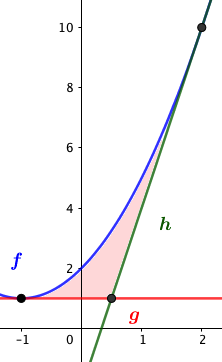
\includegraphics[width=.30\textwidth]{imagenes/imagenes08/T08IM28.png}
	\end{figure}
\end{multicols}

Hemos pues de calcular el área de la función limitada por la funciones $f$, $g$ y $h$. Una gráfica nos ayudará.

Cortes de $f$ con $g; \to (-1,1)$; cortes de $g$ con $h\;  \to (1/2,1)$; cortes de  $f$ con $h\; \to (2,10)$. Así pues, y con ayuda de la gráfica decidimos que:

$A=\displaystyle \left| \int_{-1}^{1/2} (f(x)-g(x))\; \dd x \right| \; + \; \left| \int_{1/2}^{2} (f(x)-h(x))\; \dd x \right| \; = \left| \int_{-1}^{1/2} (x^2+2x+1) \; \dd x \right| \; + \; \left| \int_{1/2}^{2} (x^2+4x+4) \; \dd x \right| = \eval[x^3/3+x^2+x|_{-1}^{1/2} + \eval[x^3+2x^2+4x|_{1/2}^{2}=\cdots= \frac 9 4 \; u^2$

\end{proofw}

\begin{ejre}
Sabiendo que el área comprendida entre las curvas $y=x^2$ e $y=kx$ es de $\dfrac 9 2 \; u^2$	, calcula $k$
\end{ejre}

\begin{proofw}\renewcommand{\qedsymbol}{$\diamond$}	

Llamamos $f$ a la primera función y $g$ a la segunda	 y buscamos donde se cortan: $f=g \to x^2=kx \to x^2-kx=x(x-k)=0 \Rightarrow x=0 \; \wedge \; x=k$. Entonces,

$A=\displaystyle \left| \int_0^k (x^2-kx)\; \dd x \right|= \eval[x^3/3 -kx^2/2|_0^k= \left|(0)-(k^3/3-k^3/2) \right| = | |k^3/6|=9/2 \Rightarrow k^3/6=\pm 9/2 \to k=3 \; \vee \; k=-3 $
\end{proofw}


\begin{ejre}
	Sea $F(x)=\displaystyle \int_1^x \cos^2 t \; \dd t$. Encuentra los posibles extremos de $F(x)$ en la `primera vuelta' ($\; [\; 0\; ,\; 2\pi]\; $).
\end{ejre}

\begin{proofw}\renewcommand{\qedsymbol}{$\diamond$}	

Por el TFCI, $F'(x)=\cos^2(x)$, sus únicos puntos críticos (como siempre existe $F'(x)$), provendrán de $F'(x)=0=\cos^2 x \Rightarrow x=\pi/2 \; \wedge \; x= 3\pi/2\; $ \textcolor{gris}{Averigüe el lector si se tratan de máximos o mínimos}

\end{proofw}

\begin{ejre}

Encuentra los puntos de derivada nula de la función $f(x)=-2x+\displaystyle \int_0^{2x} e^{t^2-10t+24}\; \dd t$	
\end{ejre}
\begin{proofw}\renewcommand{\qedsymbol}{$\diamond$}	
	
	Llamemos $g(x)=\displaystyle \int_0^{2x} e^{t^2-10t+24}\; \dd t$. Por la regal de Barrow, $g(x)=G(2x)-G(0)$, siendo $G'(x)=e^{t^2-10t+24}$
	
	Derivando: $g(x)=G(2x)-G(0) \to g'(x)= \left[ G(2x)-G(0) \right]'=G'(2x)\cdot 2 -0 =2 e^{2x^2-200x+24}$
	
	Finalmente: $f(x)=-2x+g(x) \Rightarrow f'(x)= -2+2 e^{2x^2-200x+24}$
	
	Si $f'(x)=0\to 2=2 e^{2x^2-200x+24} \to 2x^2-200x+24=0 \Rightarrow x=2 \; \wedge x=3$
\end{proofw}



\begin{ejre}
	Encuentra el área limitada por $f(x)=x^3-2x^2+x$ con la recta tangente en su máximo.
\end{ejre}

\begin{proofw}\renewcommand{\qedsymbol}{$\diamond$}	

Hemos de calcular el área encerrada entre dos funciones $f$, el polinomio que nos dan, y $g$ la recta tangente a $f$ en su máximo.

Busquemos el máximo de $f(x):\to f'(x)=3x^2-4x+1;\; f''(x)=6x-4 \quad PC(f'(x))\to y'=3x^2-4x+1=0 \to x=1 \; \wedge \; x=1/3$. Usando el criterio de la segunda derivada: $f''(1)=2>0 ;  \text { min en }  x=1 \quad f''(1/3)=-2<0 ;\text { max en }  x=1/3	$

Busquemos ahora la recta tangente a $f(x)$ en $x=1/3 \to y-f(1/3)=f'(1/3)\cdot (x-1/3) \to y=\dfrac 4 {27}=g(x)$

Encontremos ahora los `nodos' o puntos de corte de $f$ y $g$: $\; x^3-2x^2+x=\frac 4 {27} \to x=1/3 \; \wedge \; x=4/3$, por lo que:

$A=\displaystyle \left| \int_{1/3}^{4/3} (x^3-2x^2+x-\frac 4 {27})\; \dd x \right|= \cdots = \frac 1 {12} \; u^2 $ 
\end{proofw}

\begin{ejre}
$\divideontimes\;$Sea $F(x)=\begin{cases} \cos x & x<0 \\ 1 & x=0 \\ \frac 1 x \int_0^x e^{t^2}\dd t & x>0 \end{cases}\; $. Se pide:

$a)\; $ Demuestra que $F$ en ctna. en $\mathbb R$; $\; b)\; $ Estudia si existe $F'(0)$; $\; c)\; $ Estudia la continuidad de $F'(x)$
\end{ejre}
\begin{proofw}\renewcommand{\qedsymbol}{$\diamond$}	
Procedamos:

$a)\; $ El único punto conflictivo es $x=0$, veamos si $F$ es ctna. en $0$:

$F(0^-)=\underset{x_0^-}{lim}{F(x)}=1$

$F(0^+)=\underset {x\to 0^+}{lim }{F(x)}= \underset {x\to 0^+}{lim }{\dfrac {\int_0^x e^{t^2}\dd t}{x}}=(TFCI)= \underset {x\to 0^+}{lim }{\dfrac{e^{x^2}}{x}}=1$

$F(0)=1\; $.  Luego, sí, F(x) en ctna. en $x=0$ y, por tanto, ctna. en todo $\mathbb R$.

$b)\; $ $\text{Si } x<0\to F'(c)=-\sin x; \; \text{ si } x>0 \to F'(x)=\left(\dfrac {\int_0^x e^{t^2} \dd t}{x}\right)'$, existe por tratarse de dos funciones derivables y el denominador no se anula.

Para estudiar $F'(0)$, calcularemos las derivadas laterales y veremos si coinciden:

$F'(0^-)=-\sin 0 =0$

$F'(0^+)=\underset {h\to 0^+}{lim}{\dfrac {F(h)-F(0)}{h}}= 
\underset {h\to 0^+}{lim}{\dfrac {\int_0^h e^{t^2} \dd t - 1}{h^2}}= \underset {h\to 0^+}{lim}{\dfrac{e^{h^2}-1}{h^2}}=(L'H)=$

$=\underset {h\to 0^+}{lim}{\dfrac{2he^{h^2}}{h}}=0$

Como $F(0^-)=0=F(0^+)\Rightarrow \exists \; F'(0)=0$

$c)\; $
$F'(x)=\left\{ \begin{matrix}  -\sin x & x<0 \\ 0 & x=0 \\ \dfrac {x e^{x^2}-\int_0^x e^{t^2} \dd t}{x^2} & x>0  \end{matrix} \right. \quad$  El único punto conflictivo es $x=0$.

$F'(0^-)=\underset{x\to 0^-}{lim }{F'(x)}=\underset{x\to 0^-}{lim }{-\sin x }= - \sin 0 = 0$

$F'(0^+)=\underset{x\to 0^+}{lim }{F'(x)}= \underset{x\to 0^+}{lim }{ \dfrac {x e^{x^2}-\int_0^x e^{t^2} \dd t}{x^2} }= (L'H)=\underset{x\to 0^+}{lim } \dfrac {e^{x^2}+2x^2e^{x^2}-e^{x^2}}{2x}=\underset{x\to 0^+}{lim } {xe^{x^2}}=0$

Como $F'(0)=0 \Rightarrow \quad F'(x)\; $ es ctna. en $x=0$, ergo lo es en todo $\mathbb R$. 

	
\end{proofw}

\begin{ejre}
Calcula la longitud de la curva $y=x^{3/2}$ en $[0,4]$.	
\end{ejre}

\begin{proofw}\renewcommand{\qedsymbol}{$\diamond$}	

$y=f(x)=x^{3/2} \to y'=f'(x)=\frac 3 2 \; x^{1/2}$, entonces:

$l\;(\Gamma)=\displaystyle \int_0^4 \sqrt{1 + \left[ \frac 3 2 \; x^{1/2} \right]^2} \; \dd x =\left(\frac 4 9\right) \;  \int_0^4 \left(\frac 9 4\right)  \; \sqrt{1+ \frac {9x}{4}}\; \dd x= \frac 4 9 \; \eval[ \left(\frac 2 3  \left(1+ \frac {9x}{4} \right)^{3/2} \right)|_0^4 \approx 9.07\; u$ 
	
\end{proofw}

\begin{ejre}
Calcula la longitud de una semicircunferencia centrada en el origen y de radio $1\; u$.	
\end{ejre}

\begin{proofw}\renewcommand{\qedsymbol}{$\diamond$}	
$x^2+y=2=1^2 \to y=f(x)=+\sqrt{1-x^2}; \quad f'(x)=\dfrac {-x}{\sqrt{1-x^2}}	$

$l\; (\Gamma)=\displaystyle \int_{-1}^1 \sqrt{1+ \left(\dfrac {-x}{\sqrt{1-x^2}} \right)^2}\; \dd x = \int_{-1}^1 \dfrac {1}{\sqrt{1-x^2}}\; \dd x= \eval[\arcsin x|_{-1}^{1}=\pi/2-(-\pi/2)=\pi \; u$
\end{proofw}

\begin{ejre}
	Calcula los volúmenes de revolución, al girar $2\pi$ radianes alrededor de $OX$ las funciones siguientes en los intervalos que se indican:
	
$a)\; f(x)=1-x^2; \; \text{ en } [-1,1]; \qquad  b)\; g(x)=3; \; \text{ en } [0,5]$
\end{ejre}

\begin{proofw}\renewcommand{\qedsymbol}{$\diamond$}	

$a) \quad  V=\displaystyle \pi \; \int_{-1}^{1} (1-x^2)^2 \; \dd x = \pi \;  \int_{-1}^{1} (1-2x^2+x^4)\; \dd x = \pi\; \eval [x-2x^3/3+x^5/5|_{-1}^{1}= \frac {16}{15}\; \pi \; u^3$	



$b) \quad  V=\displaystyle \pi\; \int_{0}^{5} (3^2) \; \dd x= \pi\; \eval [9x|_{0}^{5}=45\:\pi\; u^3$	
\end{proofw}

\begin{ejre}
\label{cono}
	Justificar, mediante cálculo integral, que el volumen y el área lateral de un cono circular de radio $r$ y altura $h$ (generatriz $g=\sqrt{r^2+h^2}$) son: 
	
	\hspace{15mm} $V=\frac 1 3 \pi r^2 h; \quad A_L= \pi r g$
\end{ejre}
\begin{proofw}\renewcommand{\qedsymbol}{$\diamond$}	


		
Como la curva que describe el cono es la recta: $y(x)=\frac r h \; x ; \quad \text{ en } [0,h]; \quad \left(y'=\frac r h  \right)$

$V=\displaystyle \pi\; \int_0^h \left( \frac r h \; x\right)^2 \; \dd x = \pi\;\frac {r^2}{h^2} \int_0^h x^2 \: \dd x = \dfrac {\pi r^2}{h^2} \eval[x^3/3|_0^h= \dfrac {\pi r^2 h^3}{3 h^2}=\frac 1 3 \pi r^2 h$
\begin{multicols}{2}
	\begin{figure}[H]
		\centering
		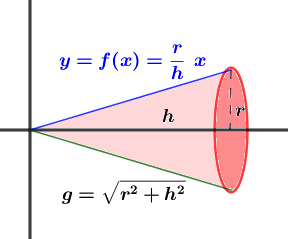
\includegraphics[width=.35\textwidth]{imagenes/imagenes08/T08IM30.png}
	\end{figure}


$A_L=2\pi \displaystyle \int_0^h f(x)\; \sqrt{1+(f'(x))^2}\; \dd x = 2 \pi \int_0^h \frac r h \; x \sqrt{1+\left(\frac r h \right)^2}\; \dd x= 2\pi \frac r h \frac {\sqrt{r^2+h^2}} h\cdot  $

$\displaystyle \cdot \int_0^h x \; \dd x = \dfrac {2 \pi r g}{h^2} \eval [x^2/2|_0^h= \dfrac {2 \pi r g}{h^2} \cdot \dfrac {h^2}{2}=$

$= \pi r g$
\end{multicols}
\end{proofw}




\textbf{\underline{Ejercicios propuestos}}.

\begin{enumerate}

\item Usando las sumas de Riemann, calcula $\displaystyle \int_0^2 (2x+1)\; \dd x$	

\rightline{\textcolor{gris}{Sol:$6$ }}

\item Sea $f$ ctna. es $[2,3]$ y $F$ una primitiva de $f$ tal que $F(2)=1$ y $F(3)=2$, Calcula:

$a)\; \displaystyle \int_2^3 f(x)\dd x;\quad b)\; \int_2^3 (5f(x)-7))\dd x; \quad c)\; \int_2^3 (F(x))^2 \dd x $

\rightline{\textcolor{gris}{Sol: $a)\; 1; \quad b)\; -2; \quad c)\; 7/3 $}}

\item Calcula el valor medio de las función $f(x)=4x^2-2x$ en $[1,4]$, así como el punto o puntos donde se alcanza.

\rightline{\textcolor{gris}{Sol:$\; <\; f \; >=69; \quad c\approx 2.66 $ }}

\item  ?`Se puede aplicar el TVM del Cálculo integral a la función $f(x)=\dfrac {x}{\sqrt{1+x^2}}$ en el intervalo $[0,1]$? En caso afirmativo, calcula el (los)  $c$ que asegura(n) que existe(n) el teorema.

\rightline{\textcolor{gris}{Sol: Sí$\quad c=\sqrt{\frac {\sqrt{2}-1}{2}}$ }}
%5
\item Sea $f(x)=|\cos x|$, definida en $[-\pi,\pi]$. Aplíquese, si es posible, el Teorema del Valor del Cálculo integral.

\rightline{\textcolor{gris}{Sol: $c=\arccos(2/\pi)$}}

	

\item Si $\displaystyle \int_0^1 f(t)\dd t=4/3; \; \int_1^2 f(t)\dd t=8/3; \;\int_0^3 f(t)\dd t=11/3\; $, Calcula:

$a)\quad \displaystyle \int_0^2 f(t)\dd t; \qquad b) \quad \int_1^3 f(t)\dd t; \qquad c) \quad \int_2^3 f(t)\dd t$

\rightline{\textcolor{gris}{Sol:$a)\; 4; \quad b)\; 7/3; \quad c) \; -1/3$ }}

\item Se sabe que: $\displaystyle \int_1^2 \left( f(x)+g(x) \right)\; \dd x=3, \quad \int_2^3 3\left( f(x)-g(x) \right)\; \dd x=3, \quad \int_1^3 f(x)\; \dd x=3 \text { y } \int_1^2 2f(x)\; \dd x=3$. Calcula, si es posible, $\displaystyle \int_1^3
g(x)\; \dd x$.

\rightline{\textcolor{gris}{Sol: Sí, el valor es $2$}}


\item Calcula las derivadas de las siguientes funciones:

\begin{multicols}{2}
\begin{enumerate}[a) ]
\item $F(x)=\displaystyle \int_{0}^{x} \cos t \; \dd t$
\item $G(x)=\displaystyle \int_{3}^{x} (t^2+1)^4 \; \dd t$
\item $H(x)=\displaystyle \int_{0}^{x} e^{-t^2} \; \dd t$
\item $I(x)=\displaystyle \int_{3}^{5} (t^2+1)^4 \; \dd t$
\item $J(x)=\displaystyle \int_{0}^{x} \cos (t^2) \; \dd t$
\item $L(x)=\displaystyle \int_{x}^{0}  (1+3t^2) \; \dd t$
\end{enumerate}	
\end{multicols}

\rightline{\textcolor{gris}{Sol: $F'(x)=\cos x; \quad G'(x)=((x^2+1)^4; \quad H'(x)=e^{-x^2};$}}

\rightline{\textcolor{gris}{$ I'(x)=0\; \quad  J'(x)=\cos (x^2); \quad L'(x)=-1-3x^2$ }}

\item Encuentra las derivadas de las funciones:
$a)\quad \displaystyle \int_1^a \dfrac {x}{1+t}\; \dd t; \qquad b) \quad \int_1^x \dfrac {x}{1+t}\; \dd t$

\rightline{\textcolor{gris}{Sol:$\; a)\; F'(x)=\int_1^a \frac {1}{1+t} \dd t; \qquad  b) \; F'(x)=\int_1^x \frac {1}{1+t} \dd t + \frac {x}{1+x}$}}
%10
\item Encuentra donde tiene extremos relativos la función $F(x)=\displaystyle \int_1^x \cos^2 t\; \dd t$

\rightline{\textcolor{gris}{Sol: $\; \pi/2\; $ y $\; 3\pi/2$}}

\item Determina un polinomio $P(x)$, de segundo grado, sabiendo que $P(0)=P(2)=1\;  \text { y } \; \displaystyle \int_0^2 P(x)\; \dd x =\dfrac 1 3 \; u^2$
 
\rightline{\textcolor{gris}{Sol: $P(x)=\frac {5x^2-10x+4}{4}$}}

\item Calculas las siguientes integrales definidas
\begin{multicols}{2}
\begin{enumerate}[a) ]
\item $\displaystyle \int_{-1}^{1} x(x^2-1) \; \dd x$
\item $\displaystyle \int_{\pi/4}^{\pi/3} \cos x \; \dd x$
\item $\displaystyle \int_{0}^{4} \sqrt{x} \; \dd x$
\item $\displaystyle \int_{0}^{\pi} \sin (2x-1) \; \dd x$
\item $\displaystyle \int_{-1}^{1} \dfrac {3}{x^2+1} \; \dd x$
\item $\displaystyle \int_{-2}^{2} e^{-x} \; \dd x$
\item $\displaystyle \int_{e}^{e^2} \dfrac {\mathrm{ln} x}{x} \; \dd x$
\item $\displaystyle \int_{0}^{\pi/4} \tan x \; \dd x$
\item  $\displaystyle \int_{1}^{1}  \dfrac {e^t}{e^{2t}+3e^t+2} \; \dd t$
\item $\displaystyle \int_0^2 \dfrac {\dd x}{x^2+4x+3}$
\end{enumerate}	
\end{multicols}

\rightline{\textcolor{gris}{\scriptsize{Sol: $a)\; 0 \quad b)\; (\sqrt{3}-\sqrt{2})/2 \quad c)\; 16/3 \quad d)\; 0 \quad e)\; 3\pi /2    \quad f)\; e^2-e^{-2} \quad g)\; 3/2 \quad h) \; 1/2 \; \mathrm{ln} 2 \quad i); \mathrm{ln}\frac {3(e+1)}{2(e+2)}; j)\; 2\mathrm{ln}2+5/6$ }}}



\item Considera la función $f(x)=\begin{cases}	
x^2 & \text{ si } -2\le x < 0 \\ 	
2x & \text{ si } 0\le x < 2 \\ 
10-3x & \text{ si } 2<x\le 4
\end{cases}$

Calcula: $\; a) \; \displaystyle \int_{-2}^1
f(x) \dd x ; \quad b) \; \int_1^4 f(x) \dd x ; \quad c)\; \int_{-2}^4 f(x) \dd x$

\rightline{\textcolor{gris}{Sol: $a)\; 11/3; \quad b) \; 5; \quad c) \; 26/3$}}

\item calcula $\displaystyle \int_0^3 |x^2-x|\; \dd x$

\rightline{\textcolor{gris}{Sol: $\; 29/6$ }}

%15
\item Calcula $\displaystyle \int_0^2 \left( 2x+|x^2-1| \right)\; \dd x$

\rightline{\textcolor{gris}{Sol: $6$ }}


\item ?`Se puede calcular la integral $\displaystyle \int_0^2 f(x)\; \dd x$, siendo $f(x)=\begin{cases}
x & 0\le x < 1 \\
x-2 & 1\le x \le 2	
\end{cases}$?. En caso afirmativo, calcúlese su valor.

\rightline{\textcolor{gris}{Sol: Si, $\; 0$ }}


\item Calcula los valores de $a$ y $b$ para que $f(x)$ sea ctna. y calcula, después $\displaystyle \int_{-1}^2 f(x) \; \dd x$

\hspace{10mm} $f(x)=\begin{cases}
2^x+a & x\le -1 \\ 	ax+b & -1<x\le 0 \\ 3x^2+2 & x>0
\end{cases}$


\rightline{\textcolor{gris}{Sol: $\; a=3/4;\quad b=2; \quad integral=-109/8$ }} 


\item Calcula, si existen, las siguientes integrales impropias.
\begin{multicols}{2}
\begin{enumerate}[a) ]
\item $\displaystyle \int_{0}^{+\infty} e^{-x}\; \sin x \; \dd x\; $ (Partes)
\item $\displaystyle \int_{-\infty}^1{} x\; e^x \;  \dd x\; $ (Partes)
\item $\displaystyle \int_{1}^{+\infty} \cos x \;  \dd x\; $ (Inmed.)
\item $\displaystyle \int_{4}^{+\infty} \dfrac {1}{x^2-4}\;  \dd x\; $ (Racional)
\item $\displaystyle \int_{1}^{+\infty} \dfrac 1 x \;  \dd x\; $ (Inmed.)
\item $\displaystyle \int_{-\infty}^{-2} \dfrac 1 {x^2} \;  \dd x\; $ (Inmed.)
\item $\displaystyle \int_{0^+}^{e} \dfrac {\mathrm{ln} x}{\sqrt{x}} \;  \dd x\; $ (Discont: $0$; Partes)
\item $\displaystyle \int_{0^+}^{1} x\; \mathrm{ln} x \;  \dd x\; $ (Discont: $0$; Partes)
\end{enumerate}	
\end{multicols}
\rightline{\textcolor{gris}{Sol: $a)\;1/2;\quad b); 0;\quad c)\; \nexists; \quad d)\; (\mathrm{ln}2)/2; \quad e); \nexists; \quad f); 1/2; \quad g)\; -\sqrt{e}; \quad h)\; -1/4 $}}

\item Un profesor pregunta a sus alumnos que calculen $\displaystyle \int_{-3}^2 \dfrac {\dd x}{x^2}$

La alumna $\alpha$ trabajó así: 
$\displaystyle \int_{-2}^3 \dfrac {\dd x}{x^2}= \eval[-\dfrac 1 x|_{-3}^2=-\frac 1 2 -\left(-  \frac 1 {-3} \right)=-\frac 5 6$

Y luego razonó: ``Estoy segura de que algo está mal porque sé que la función $f(x)=\dfrac 1 {x^2} $ es positiva  en todo su dominio, por lo que $\displaystyle \int_{-2}^3 \dfrac {\dd x}{x^2}$ no puede ser negativa''.

?`Dónde está el error?

\rotatebox{180}{\leftline{\textcolor{gris}{\scriptsize{Sol: $\frac 1 {x^2}$ no está definida en $x0=\in [-3,2]$}}}}


%20
\item Calcula el área encerrada por $y=x^2+x-2$ con $OX$ en $[-1,4]$

\rightline{\textcolor{gris}{Sol: $\; 155/6 \; u^2$}}


\item Calcula el área encerrada por $f(x)=\mathrm{ln} x$, las rectas $y=0 \quad x=2\quad x=2\sqrt{3}$

\rightline{\textcolor{gris}{Sol: $\; 6\mathrm{ln}6-\frac 1 2 \mathrm{ln}2- \frac 9 2 \; u^2$}}

\item Calcula el area comprendida entre las siguientes funciones: 
\begin{multicols}{2}
\begin{enumerate} [a) ]
\item $y=x^2 \; \quad y=1$
\item $y=-x^2+4x-4; \quad y=2x-7$
\item $y=x(x-1)(x-2); \quad y=0$
\item $y=x^2-2x; \quad y=-x^2+4x$
\end{enumerate}	
\end{multicols}
\rightline{\textcolor{gris}{Sol: $a)	\; 1/2 \; u^2 \quad b) \; 32/2 \; u^2 ; \quad c)\; 1/2 \; u^2; \quad d)\; 9 \; u^2$}}
\item Sean $a=\displaystyle \int_0^{\pi/2} x \sin^2 x \dd x$ y $b=\displaystyle \int_0^{\pi/2} x \cos^2 x \dd x$. Calculando previamente $a+b$ y $a-b$, determina los valores de $a$ y $b$.
 

 \rightline{\textcolor{gris}{Sol: $\; a= \frac {\pi^2+4}{16}; \quad b= \frac {\pi^2-4}{16}$}}
 
 \item Calcula el área del recinto limitado por la gráfica de la función $f(x)=\dfrac {1}{x(^2+1) }$, el eje $x$ y las rectas $x=1$ y $x=\sqrt{3}$
  
 \rightline{\textcolor{gris}{Sol: $ \frac 1 2 \mathrm{ln}\frac 3 2$}}
 %25
\item Sea $f(x)=x\; |x-2|$, calcula el área que encierra con $OX$.

\rightline{\textcolor{gris}{Sol: $4/3 \; u^2$}}
 
 \item Dibuja el recinto limitado por las siguientes curvas y calcula su área en el intervalo $[0,2\pi]$, siendo $f(x)=2\sin x$ y $g(x)=\sin(2x)$
 
\rightline{\textcolor{gris}{Sol: $ 8\; u^2$}}

\item Sea $f(x)=\begin{cases}
4x & 0\le x \le 1 \\
\dfrac {16}{(x+1)^2} & 1<x<3 \\
4-x & 3\le x \le 4
\end{cases}\; $.  Calcula el área encerrada por $f(x)$ con $OX$.

\rightline{\textcolor{gris}{Sol: $ 13/2 \; u^2$}}

 
 \item Calcula el área de la región del semiplano $y\ge 0$ limitado lor la curva $y=\mathrm{ln}x$, su tangente en $x=1$ y la recta $x=3$.
 
\rightline{\textcolor{gris}{Sol: $4-\mathrm{ln}3$}}

\item Calcula el área limitada por las parábolas $y=x^2$ e $y=\sqrt{x}$

 \rightline{\textcolor{gris}{Sol: $ 1/3$}}
 
% 30
 \item Hallar el áres $A(\lambda)$ limitada por las gráficas $f(x)=\dfrac 1 x$ y $g(x)=\dfrac 1 {\sqrt{x}}$ entre los valores $x=1$ y $x=\lambda >1$, y hallar el límite de $A(\lambda)$ cuando $\lambda \to + \infty$

 \rightline{\textcolor{gris}{Sol: $ A(\lambda )=2\sqrt{\lambda}+ \frac 1 {\lambda}-3; \quad \underset {\lambda \to + \infty}{ lim }\; A(\lambda)=+\infty $ }}
 
 \item Calcula el área limitada por las curvas $y^2=x$ e $y=|x-2|$.
  
 \rightline{\textcolor{gris}{Sol: $16/3\; u^2$}}
 
 \item Sea $a\in ]0,1[$, la función $f_a(x)=\dfrac {1-a}{a^2}\; x^2$ es una parábola que pasa por los puntos $(0,0)$ y $(a,1-a)$. Calcula $A(a)$, área de la región limitada por $f_a$, $OX$ y las verticales $x=0$ y $x=a$, y calcula el valor de $a$ para el cuál $A(a)$ es máxima.
 
\rightline{\textcolor{gris}{Sol: $A(a)=\frac 1 3 (a-a^2); \quad A_{max} \leftrightarrow a=1/2$}}


\item Sean $f(x)=6-x^2$ y $g(x)=|x|$. Dibuja el recinto limitado por ambas curvas y calcula su área.

\rightline{\textcolor{gris}{Sol: $44/3: u^2$}}


\item Sea $f(x)=e^{-x/2}$. Encuentra el área encerrada por $f(x)$, su recta tangente en el punto de abcisa $x=0$ y la vertical $x=2$.

\rightline{\textcolor{gris}{Sol: $(1-\frac 2 e)\; u^2$}}

 %35
\item El área del recinto limitado por las curvas $y=\dfrac {x^2}{a}$ e $y=\sqrt{ax}$, con $a>0$, vale $3\; u^2$. Calcula el valor de $a$.

\rightline{\textcolor{gris}{Sol: $a=3$}}


\item Sea $f(x)=\begin{cases} ax^2+b & |x|<2 \\ \dfrac 1 {x^2} & |x|\ge 2 \end{cases}$. se pide:

\vspace{3 mm}

\hspace{10mm} $a) \quad$ Los valores de $a $ y $b$ para que $f$ sea ctna. y dvble. en todo $\mathbb R$

\hspace{10mm} $b) \quad$ Para eos valores obtenidos, determina el área encerrada por $f(x)$ con $OX$, y las rectas $y=0$, $x=1\; $ y $\; x=3$

\rightline{\textcolor{gris}{Sol: $a=-1/16; \; b= 1/2; \quad \text{Área }=25/48 \; u^2$}}


\item Encuentra el área del recinto limitado por el eje $X$, la función $y=e^{-x}$ y las rectas tangente y normal a $f(x)$ en $x=-1$

\rightline{\textcolor{gris}{Sol: $\; \frac {e^3+e}{2}\; u^2$}}

\item Calcula la longitud de la `catenaria' $y=\dfrac {e^x+e^{-x}}{2}$ entre $x=-1$ y $x=1$. (\scriptsize{Ayuda: como y es par, puedes calcular la long. desde $0$ a $1$ y multiplicar por $2$; dentro de la raíz del radicando, al desarrollar los cálculos, aparece un `trinomio perfecto', que se puede escribir como el cuadrado de un binomio, lo que simplifica la integral)}\normalsize{.}

\rightline{\textcolor{gris}{Sol: $\; (e-\frac 1 e) \; u$}}


\item Calcula las siguientes longitudes de arcos:

$a)\; f(x)=\dfrac {(4x-3)\sqrt{x}}{6}; \; \text { en } [1,9]\; ; \qquad b)\; g(x)=\dfrac {x^4}{8} + \dfrac {1}{4x^2}, \; \text { en } [1,3]$

\rightline{\textcolor{gris}{Sol: $a)\;  \frac {55}{3}\; u; \quad b)\; \frac {92}{2} \; u$}}
%40
\item Calcula la longitud del arco que tiene por ecuaciones paramétricas:

$w(t)=\begin{cases} x=e^t\;  \sin t \\ y= t\;  \cos t \end{cases}; \quad 0\le t \le \pi $

\rightline{\textcolor{gris}{Sol: $\sqrt{2}(e^{\pi}-1)\; u$}}

\item $a)$ Calcula el volumen engendrado por $y=-x^2+4$, con $-2\le x \le 1$, al girar alrededor de $OX$

$b)$ Calcula el volumen engendrado por $y=-x^2+4$, con $-2\le x \le 2$, al girar alrededor de $OY$

\rightline{\textcolor{gris}{Sol: $\;a)\; 30.6 \; \pi \; u^3; \quad b)\; 16\; \pi\; u^3$}}

\item Calcula el volumen del elipsoide e revolución que se obtiene al girar alrededor de $OX$ la elipse $\dfrac{x^2}{25}+\dfrac{y^2}{16}=1$

\rightline{\textcolor{gris}{\footnotesize{Despeja y(x)>0, los límites de integración se obtienen al hacer $y=0\leftrightarrow x=\pm 5$.}}}
\rightline{\textcolor{gris}{\normalsize{ La solución es: $106.67\; \pi\; u^3$}}}



\item Justificar, usando CI,  que el volumen y el áreal lateral de un tronco de cono de altura $r$ y radios $r_1$ y $r_2<r_1$ son:

\hspace{15mm} $V=\frac 1 3 \pi (r_1^2+r_1 \cdot r_2+r_2^2)h; \quad A_L=\pi (r_1+r_2) \sqrt{h^2+(r_1-r_2)^2}$

\rightline{\textcolor{gris}{(ver ejercicio resuelto \ref{cono})}}


\end{enumerate}

%\clearpage

\section{Curiosidades y aplicaciones de la ID}

\textbf{A1} \begin{figure}[H]
		\centering
		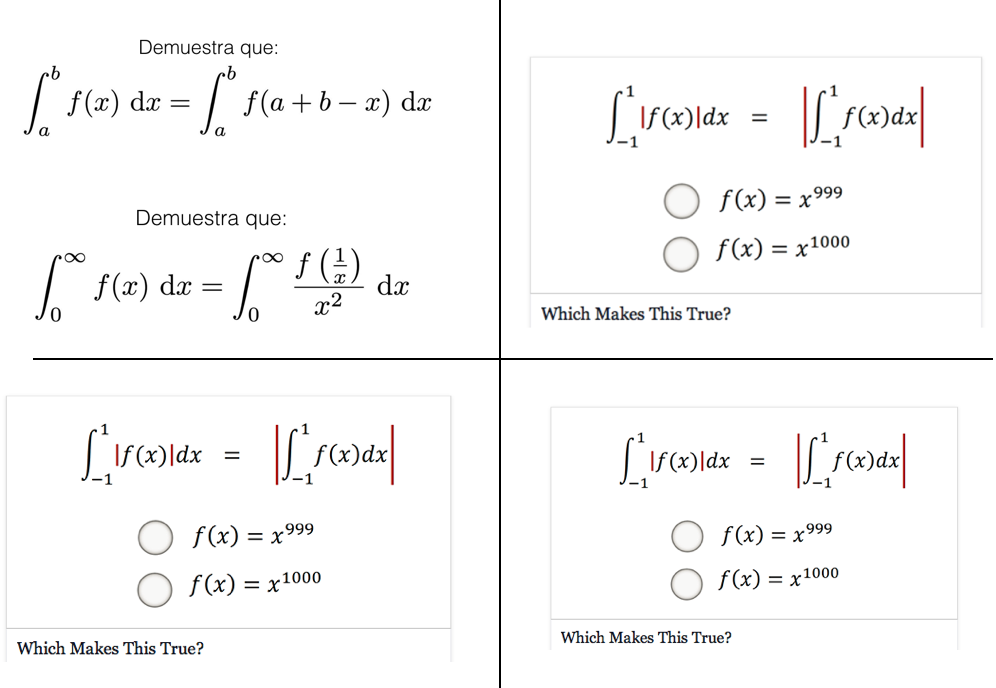
\includegraphics[width=.9\textwidth]{imagenes/imagenes08/T08IM31.png}
	\end{figure}
 

 
  \textbf{A2}  \begin{figure}[H]
		\centering
		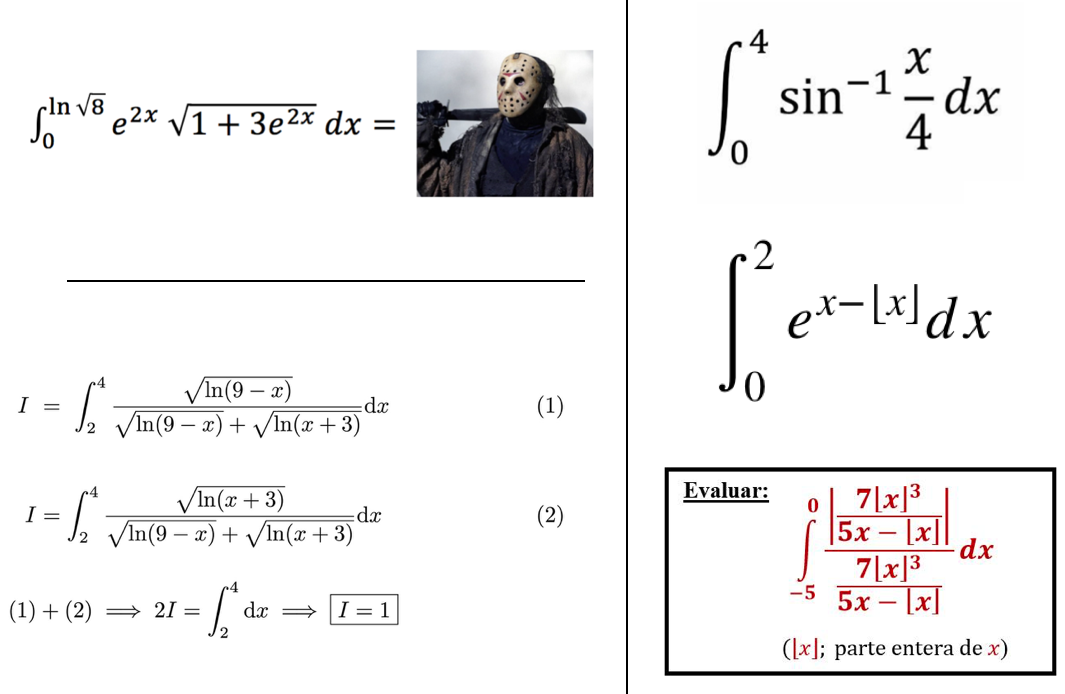
\includegraphics[width=1\textwidth]{imagenes/imagenes08/T08IM32.png}
	\end{figure}
 
 
 
 \textbf{A3}  \begin{figure}[H]
		\centering
		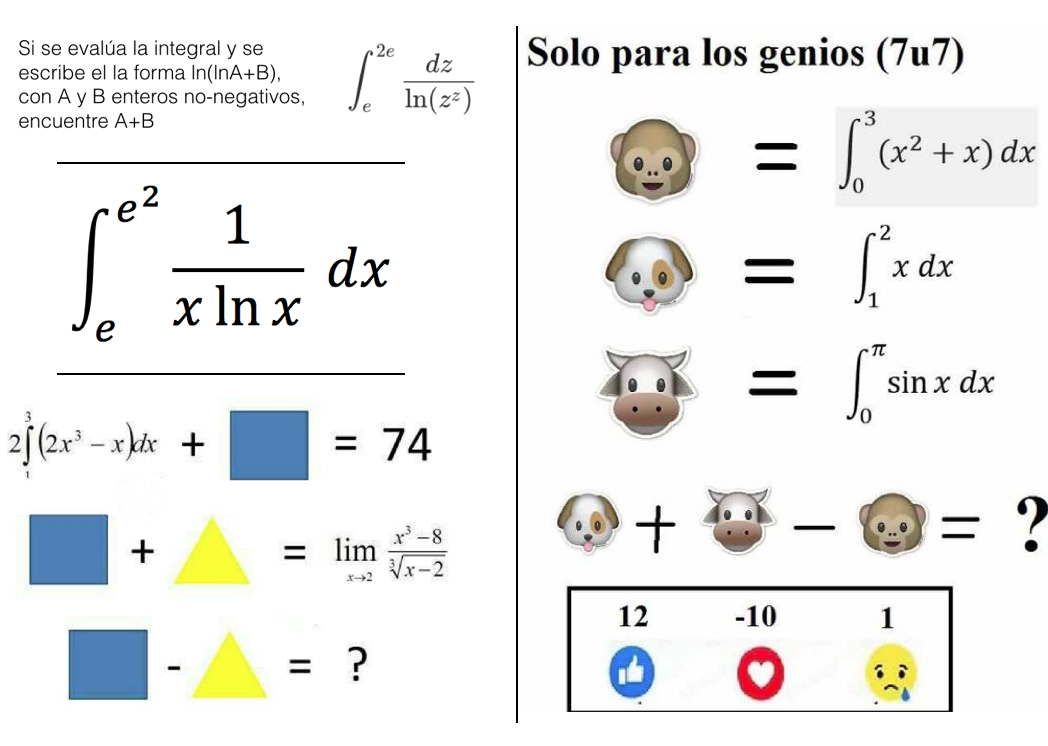
\includegraphics[width=0.9\textwidth]{imagenes/imagenes08/T08IM33.png}
	\end{figure}

$\quad$

$\quad$

	
\textbf{A4} \begin{figure}[H]
		\centering
		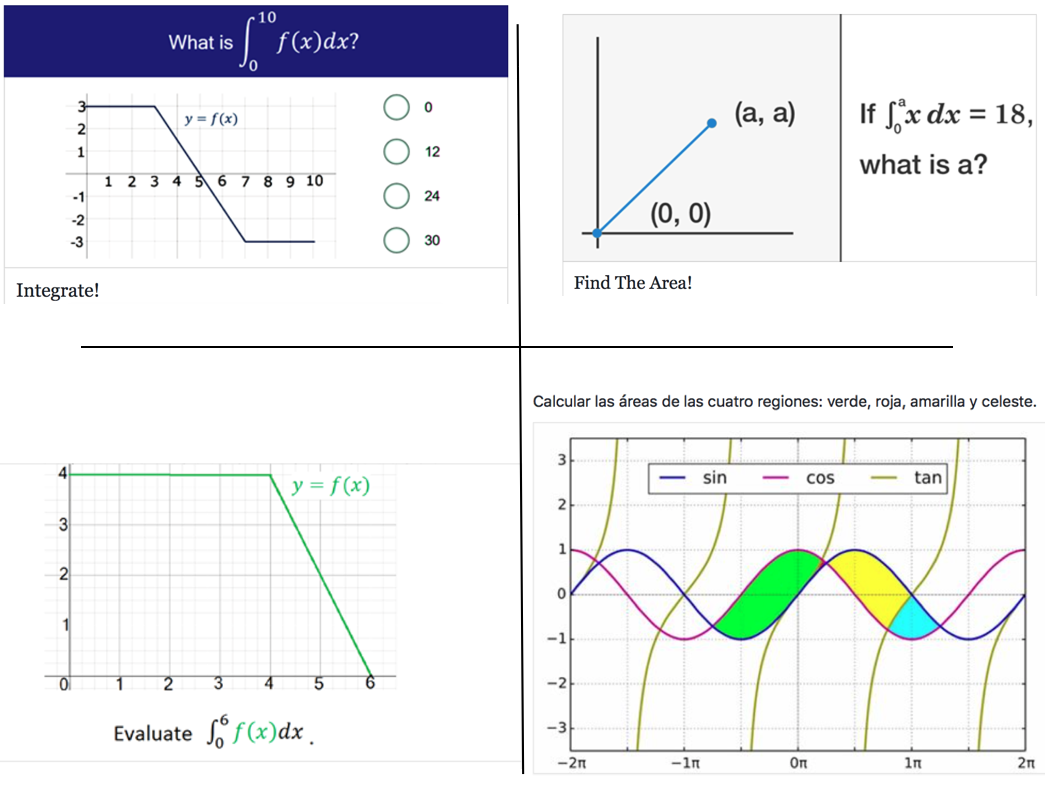
\includegraphics[width=.9\textwidth]{imagenes/imagenes08/T08IM34.png}
	\end{figure}
	

\textbf{A5} \textbf{La trompeta de Gabriel ( o de Torricelli).}

Se trata de una `aparente' paradoja en la que un cuerpo de revolución tiene volumen finito $V$, pero área infinita. Esto llevaría a que la superficie interior si se podría pintar echándole $V\; u^3$ de pintura, con lo que la superficie no sería infinita.

 	\begin{figure}[H]
		\centering
		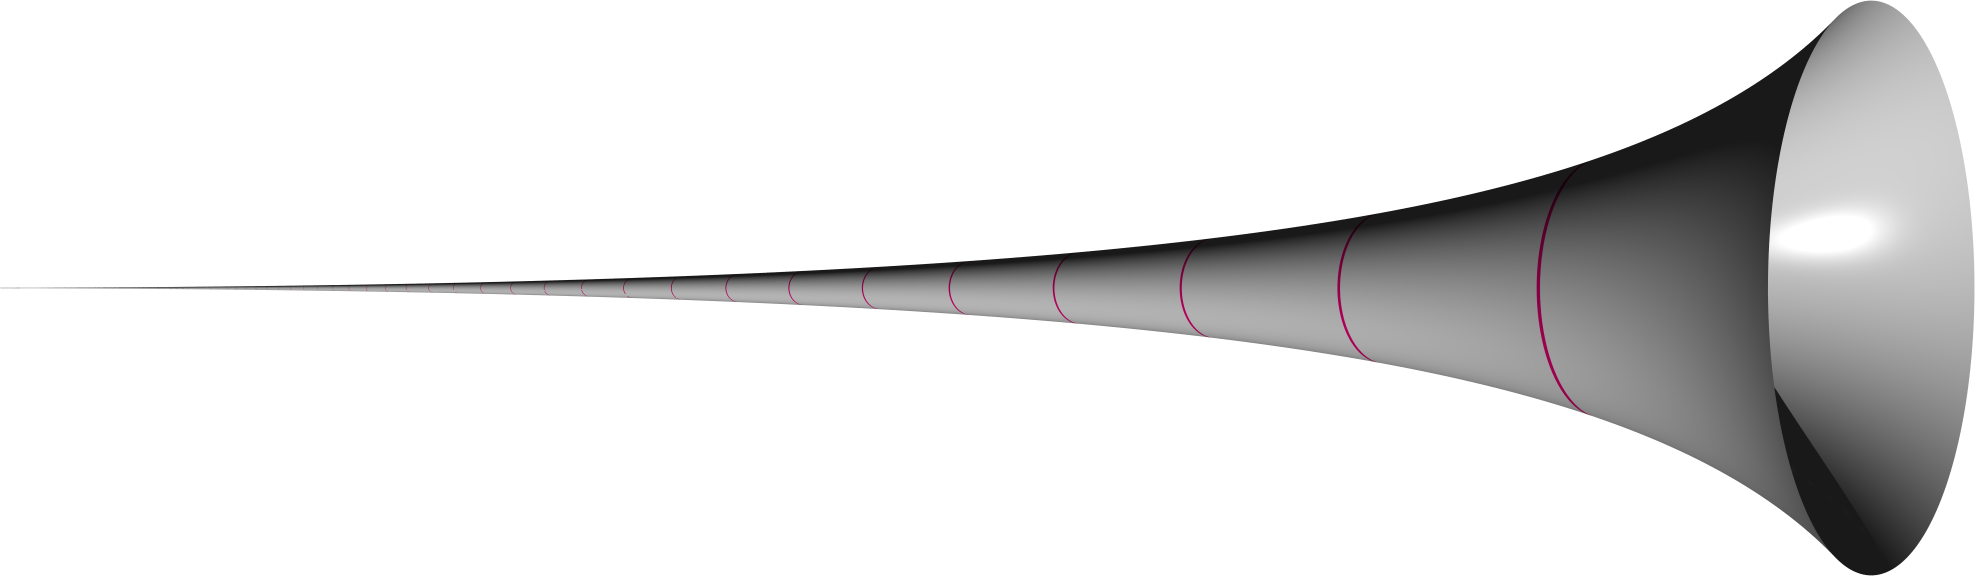
\includegraphics[width=1\textwidth]{imagenes/imagenes08/T08IM35.png}
	\end{figure}

Se trata de calcular el volumen y el área del cuerpo de revolución engendrado por la función $f(x)=\dfrac 1 x$ dese $x=1$ hasta $+\infty$.

\underline{Cálculo del área}: 

$A=\pi\; \underset{x \to +\infty}{lim}\;{\displaystyle \int_1^x \dfrac 1 t \; \dd t }= \pi\; \underset{x \to +\infty}{lim} {  \eval[\mathrm{ln}t|_1^x }= \pi\; \underset{x \to +\infty}{lim} { \mathrm{ln}x }= \infty$

$\quad$

\underline{Cálculo del volumen}:

 $V= \pi\; \underset{x \to +\infty}{lim}\;{\displaystyle \int_1^x \dfrac 1 {t^2} \; \dd t }$ 
$= \pi\; \underset{x \to +\infty}{lim} {  \eval[- \frac 1 t|_1^x }= \pi\; \underset{x \to +\infty}{lim} { -\frac 1 t + 1 }=1 \; u^3$

$\quad$

\textcolor{gris}{ En el momento de su descubrimiento, fue considerado una paradoja. Esta paradoja aparente ha sido descrita de modo informal señalando que sería necesaria una cantidad infinita de pintura para cubrir la superficie exterior, mientras que sería posible rellenar toda la figura con una cantidad finita de pintura y así cubrir esa superficie.}

\small{\textcolor{gris}{La solución de la paradoja es que un área infinita requiere una cantidad infinita de pintura si la capa de pintura tiene un grosor constante. Esto no se cumple en el interior del cuerno (o trompeta), ya que la mayor parte de la longitud de la figura no es accesible a la pintura, especialmente cuando su diámetro es menor que el de una molécula de pintura. Si se considera una pintura sin grosor, sería necesaria una cantidad infinita de tiempo para que ésta llegase hasta el``final'' del cuerno.En otras palabras, llegaría un momento en el que el espesor de la trompeta sería más pequeño que una molécula de pintura con lo que, digamos, una gota de pintura cubriría el resto de la superficie de la trompeta (aunque fuera infinito). Así, que la superficie de la trompeta sea infinita no implicaría que la cantidad de pintura tenga que ser infinita.}}

\small{\rightline{\textcolor{gris}{Fuente: Wikipedia}}}

\begin{figure}[H]
	\centering
	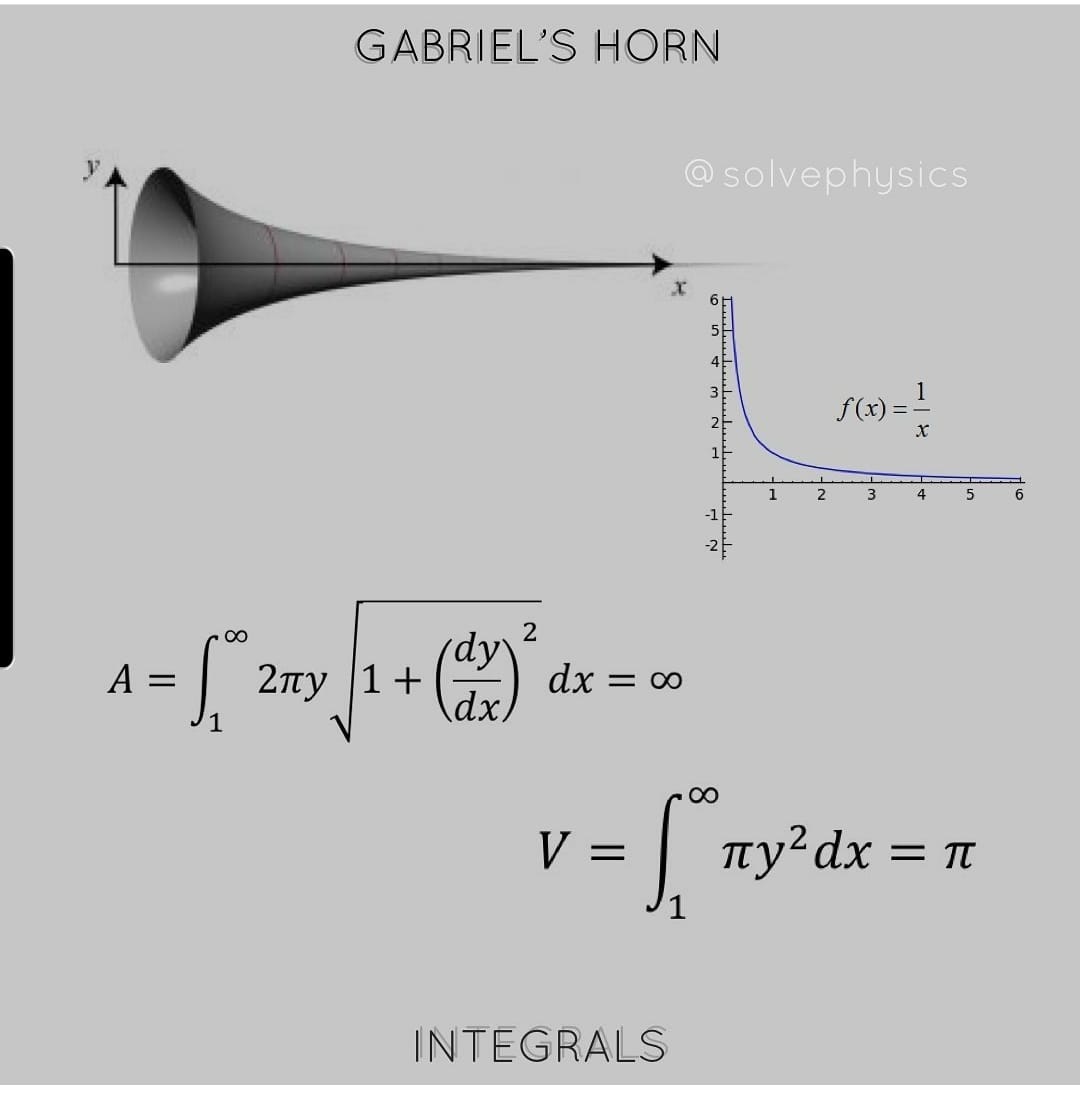
\includegraphics[width=0.8\textwidth]{imagenes/imagenes08/T08IM36.png}
\end{figure}

\textbf{A6} \textbf{Aplicaciones de la ID a otras ciencias}.

Las integrales definidas también se utilizan en probabilidad, administración, economía, ecología, computación, arquitectura, en las ingenierías  y en muchas otras ramas de las ciencias, incluidas las ciencias sociales. Veremos algunos ejemplos:

\vspace{5mm}

\begin{enumerate}[{A6} 1. ]

	\item La función $\rho (x)=300 \left[ 2+\sin(4\sqrt{x+0.15}) \right]$ da la densidad de coches (en número de coches por $km$) en los primeros $20\; km$ de una autovía, siendo $x$ la distancia en $lm$ al comienzo de la misma. Calcula el número total de coches en ls $20 \; km$.  
	
	\vspace{3mm}
	
	$\displaystyle \int_0^{20} \rho (x) \; \dd x= \int_0^{20} 300 \left [2+\sin(4\sqrt{x+0.15}) \right]   \; \dd x=$
	
	$\diamond = 600 \int_0^{20} \dd x + 300 \int_0^{20}  \sin (4\sqrt{x+0.15}) \; \dd x = \; \to $
	
	$\to \; CV:\; \left[ \begin{matrix} \sqrt { x+0.15 } =t \\ \dd x=2t\quad \dd t \end{matrix} \right] \to $
	$ \; =\cdots\; $ (\textcolor{gris}{Acábese}) $ \cdots   =11513 \text{ coches } $
	
	
	
	\vspace{5mm}
	
	\item La posición de un móvil en el plano viene dada por el par de funciones $x(t)=t^2$ e $y(t)=t+t^3/3$, donde $t$ es el tiempo transcurrido en $s$ y $x \text{ e } y$ son las posiciones que ocupa la partícula en cada instante y están expresadas en $m$. El espacio recorrido desde el instante $t=0$ hasta $t=2 \; s$ viene medido por el arco de la curva que describe el móvil. Calcúlese este espacio.
	
	\vspace{3mm}
	
	$e=l\; (\Gamma) = \displaystyle \int_0^2 \sqrt{x'(t)^2 + y'(t)^2}\; \dd t=$
	$[\;  x'(t)=2t; \quad y'=1+t^2 \;  ]$
	$\; = \int_0^2 \sqrt{2t+1+t^2}\; \dd t = \int_0^2 \sqrt{(t+1)^1}\; \dd t = \int_0^2 ((t+1)\; \dd t = \eval[t^2/2+t|_0^2= (2+2)-(0)=4\; m$
	
	\vspace{5mm}
	
	\item Sobre una partícula situada a $x\; m$ del origen, actúa una fuerza $F=(3x^2+2x)\; N$. ¿Qué trabajo realiza dicha fuerza al mover la partícula desde la posición $x=1$ hasta $x=5\; m$
	
	\vspace{3mm}
	
	Us resultado de física asegura que el trabajo $W$ que realiza un cuerpo sometido a una fuerza $F$ desde $x=x_1$ hasta $x= x=2$ es  $\; W=\displaystyle \int_{x_1}^{x_2} F \cdot \dd x $, luego:
	
	$W=\displaystyle \int_1^5 (3x^2+2x)\; \dd x = \eval[x^3+x^2|_1^5=(5^3+5^2)-(1+1)= 148\; J$. 
	
	Un $J$ es la unidad física de trabajo, $N\cdot m$
	
	\vspace{5mm}
	
	\item Calcula la posición de un móvil sabiendo que se desplaza rectilíneamente con a aceleración constante igual a $a=8 \; m\cdot s^{-2}$ y que su velocidad es $0\; m\cdot s^{-1}$ cuando $t=3 \; s$ y que se encuentra en el origen de coordenadas a los $11 \; s$
	
	\vspace{3mm}
	
	Sea $s(t)$ la posición del móvil a los $t\; s$. Por física sabemos que: $v(t)=s'(t)=\frac {\dd s(t)}{\dd t}\; $ y $\; a(t)=s''(t)=\frac {\dd^2 s(t)}{\dd t^2}=8\; m\cdot s^{-2}$
	
	Calculemos la velocidad: $v(t)=\int a(t)\; \dd t = \int 8 \dd t =8t +\mathcal {C}_1\; $; como $v(3)=0=24+\mathcal {C}_1 \to  \mathcal {C}_1=-24 \Rightarrow v(t)=8t-24$
	
	Calculemos, ahora, la posición: $s(t)=\int v(t)\; \dd t = \int (8t-24)\; \dd t = 4t^2 -24t +\mathcal {C}_2\; $; como $s(11)=0=220+\mathcal {C}_2 \to \mathcal{C}_2=-220 \Rightarrow s(t)=4t^2-24t-220$ 
	
\end{enumerate}


\textbf{A7} Cálculo de un límite.

$\boldsymbol{\underset{n\to \infty}{lim}{\left( \dfrac {n!}{n} \right) ^{1/n}}} = \underset{n\to \infty}{lim} \left( \frac 1 n \frac 2 n \cdots \frac n n\right)^{1/n}=0^0\; (ind)$

$\displaystyle L=\underset{n\to \infty}{lim}{\left( \dfrac {n!}{n} \right) ^{1/n}} \to ln \; L = ln \underset{n\to \infty}{lim}{\left( \dfrac {n!}{n} \right) ^{1/n}}= \underset{n\to \infty}{lim}ln {\left( \dfrac {n!}{n} \right) ^{1/n}}= \underset{n\to \infty}{lim} \dfrac 1 n \; ln{\left( \dfrac {n!}{n} \right)} =  \underset{n\to \infty}{lim}\dfrac 1 n \; ln {\left( \dfrac 1 n \dfrac 2 n \cdots \dfrac n n \right)} = \underset{n\to \infty}{lim}\;  \dfrac 1 n\;  \sum_{k=1}^n \; ln\left( \dfrac k n \right)=(*1)= \int_0^1 ln x \; \dd x =(*2)=\eval[x \; ln x  - x|_0^1=(*3)=-1 \to L=e^{-1}=\dfrac 1 e $


$\quad$

\small{$(1*)$} Dada la función $f(x)=ln x$, en $[0,1]$, tomamos $Pn:\; 0, 1/n, 2/n, \cdots n/n=1 \to$
$ \displaystyle \sum_{k=1}^n \dfrac 1 n \cdot \left( \dfrac k n \right) = \int_0^1 lnx\; \dd x$

$(2*)$ Integrando por partes: $\left[ \begin{matrix} u=ln\; \to \dd u= \dfrac 1 x \\ \dd v = \dd x \to v=x  \end{matrix} \right] \to \displaystyle \int ln x \; \dd x = xln x-x+\mathcal C$

$(3*)$ Integral impropia, hay que calcular $\displaystyle \underset {x\to 0}{lim} x\; ln x =\textcolor{gris}{0\infty}=\underset {x\to 0}{lim} \dfrac {ln x}{1/x}=\textcolor{gris}{\infty / \infty \to L'H}= $ 
$\displaystyle \underset {x\to 0}{lim} \dfrac {1/x}{-1/x^2}=\underset {x\to 0}{lim} (-x)=0$\normalsize{.}


	

	
